\documentclass[a4paper]{book}
\usepackage{a4wide}
\usepackage{makeidx}
\usepackage{fancyhdr}
\usepackage{graphicx}
\usepackage{multicol}
\usepackage{float}
\usepackage{textcomp}
\usepackage{alltt}
\usepackage{ifpdf}
\ifpdf
\usepackage[pdftex,
            pagebackref=true,
            colorlinks=true,
            linkcolor=blue,
            unicode
           ]{hyperref}
\else
\usepackage[ps2pdf,
            pagebackref=true,
            colorlinks=true,
            linkcolor=blue,
            unicode
           ]{hyperref}
\usepackage{pspicture}
\fi
\usepackage[utf8]{inputenc}
\usepackage{doxygen}
\makeindex
\setcounter{tocdepth}{1}
\renewcommand{\footrulewidth}{0.4pt}
\begin{document}
\begin{titlepage}
\vspace*{7cm}
\begin{center}
{\Large OWL-PHP Reference Manual\\[1ex]\large 010 }\\
\vspace*{1cm}
{\large Generated by Doxygen 1.5.4}\\
\vspace*{0.5cm}
{\small Thu Aug 7 12:18:51 2008}\\
\end{center}
\end{titlepage}
\clearemptydoublepage
\pagenumbering{roman}
\tableofcontents
\clearemptydoublepage
\pagenumbering{arabic}
\chapter{OWL-PHP Module Index}
\section{Modules}
Here is a list of all modules:\begin{DoxyCompactList}
\item \contentsline{section}{Presentation modules}{\pageref{group__OWL__UI__LAYER}}{}
\item \contentsline{section}{Business Object modules}{\pageref{group__OWL__BO__LAYER}}{}
\item \contentsline{section}{Storage Object modules}{\pageref{group__OWL__SO__LAYER}}{}
\item \contentsline{section}{Library (codes, messages files etc.)}{\pageref{group__OWL__LIBRARY}}{}
\item \contentsline{section}{Plugins for the presentation modules}{\pageref{group__OWL__UI__PLUGINS}}{}
\item \contentsline{section}{Drivers}{\pageref{group__OWL__DRIVERS}}{}
\end{DoxyCompactList}

\chapter{OWL-PHP Hierarchical Index}
\section{Class Hierarchy}
This inheritance list is sorted roughly, but not completely, alphabetically:\begin{DoxyCompactList}
\item \contentsline{section}{\_\-OWL}{\pageref{class__OWL}}{}
\begin{DoxyCompactList}
\item \contentsline{section}{baseDOMelement}{\pageref{classbaseDOMelement}}{}
\item \contentsline{section}{DataHandler}{\pageref{classDataHandler}}{}
\item \contentsline{section}{DbHandler}{\pageref{classDbHandler}}{}
\item \contentsline{section}{Dispatcher}{\pageref{classDispatcher}}{}
\item \contentsline{section}{FileHandler}{\pageref{classFileHandler}}{}
\begin{DoxyCompactList}
\item \contentsline{section}{ImageHandler}{\pageref{classImageHandler}}{}
\end{DoxyCompactList}
\item \contentsline{section}{FormHandler}{\pageref{classFormHandler}}{}
\item \contentsline{section}{LogHandler}{\pageref{classLogHandler}}{}
\item \contentsline{section}{OWL}{\pageref{classOWL}}{}
\item \contentsline{section}{SchemeHandler}{\pageref{classSchemeHandler}}{}
\item \contentsline{section}{SessionHandler}{\pageref{classSessionHandler}}{}
\begin{DoxyCompactList}
\item \contentsline{section}{Session}{\pageref{classSession}}{}
\end{DoxyCompactList}
\item \contentsline{section}{UserHandler}{\pageref{classUserHandler}}{}
\begin{DoxyCompactList}
\item \contentsline{section}{User}{\pageref{classUser}}{}
\end{DoxyCompactList}
\end{DoxyCompactList}
\item \contentsline{section}{ConfigHandler}{\pageref{classConfigHandler}}{}
\item \contentsline{section}{Form}{\pageref{classForm}}{}
\item \contentsline{section}{FormField}{\pageref{classFormField}}{}
\begin{DoxyCompactList}
\item \contentsline{section}{FormFieldButton}{\pageref{classFormFieldButton}}{}
\item \contentsline{section}{FormFieldCheckbox}{\pageref{classFormFieldCheckbox}}{}
\item \contentsline{section}{FormFieldFile}{\pageref{classFormFieldFile}}{}
\item \contentsline{section}{FormFieldRadio}{\pageref{classFormFieldRadio}}{}
\item \contentsline{section}{FormFieldSelect}{\pageref{classFormFieldSelect}}{}
\item \contentsline{section}{FormFieldText}{\pageref{classFormFieldText}}{}
\item \contentsline{section}{FormFieldTextarea}{\pageref{classFormFieldTextarea}}{}
\end{DoxyCompactList}
\item \contentsline{section}{OldOFMStuff}{\pageref{classOldOFMStuff}}{}
\item \contentsline{section}{OWLException}{\pageref{classOWLException}}{}
\item \contentsline{section}{OWLExceptionHandler}{\pageref{classOWLExceptionHandler}}{}
\item \contentsline{section}{OWLloader}{\pageref{classOWLloader}}{}
\item \contentsline{section}{Register}{\pageref{classRegister}}{}
\item \contentsline{section}{StatusHandler}{\pageref{classStatusHandler}}{}
\end{DoxyCompactList}

\chapter{OWL-PHP Class Index}
\section{OWL-PHP Class List}
Here are the classes, structs, unions and interfaces with brief descriptions:\begin{CompactList}
\item\contentsline{section}{\hyperlink{class__OWL}{\_\-OWL} }{\pageref{class__OWL}}{}
\item\contentsline{section}{\hyperlink{classDataHandler}{DataHandler} (The OWL Data object )}{\pageref{classDataHandler}}{}
\item\contentsline{section}{\hyperlink{classDbHandler}{DbHandler} (Database handler )}{\pageref{classDbHandler}}{}
\item\contentsline{section}{\hyperlink{classFileHandler}{FileHandler} (File handler )}{\pageref{classFileHandler}}{}
\item\contentsline{section}{\hyperlink{classSessionHandler}{SessionHandler} (PHP session object )}{\pageref{classSessionHandler}}{}
\end{CompactList}

\chapter{OWL-PHP File Index}
\section{OWL-PHP File List}
Here is a list of all files with brief descriptions:\begin{CompactList}
\item\contentsline{section}{/home/oscar/work/eclipse/owl-php/src/\hyperlink{config_8php}{config.php} }{\pageref{config_8php}}{}
\item\contentsline{section}{/home/oscar/work/eclipse/owl-php/src/\hyperlink{index_8php}{index.php} }{\pageref{index_8php}}{}
\item\contentsline{section}{/home/oscar/work/eclipse/owl-php/src/inc/\hyperlink{class_8__OWL_8php}{class.\_\-OWL.php} }{\pageref{class_8__OWL_8php}}{}
\item\contentsline{section}{/home/oscar/work/eclipse/owl-php/src/inc/\hyperlink{class_8datahandler_8php}{class.datahandler.php} }{\pageref{class_8datahandler_8php}}{}
\item\contentsline{section}{/home/oscar/work/eclipse/owl-php/src/inc/\hyperlink{class_8dbhandler_8php}{class.dbhandler.php} }{\pageref{class_8dbhandler_8php}}{}
\item\contentsline{section}{/home/oscar/work/eclipse/owl-php/src/inc/\hyperlink{class_8filehandler_8php}{class.filehandler.php} }{\pageref{class_8filehandler_8php}}{}
\item\contentsline{section}{/home/oscar/work/eclipse/owl-php/src/inc/\hyperlink{class_8sessionhandler_8php}{class.sessionhandler.php} }{\pageref{class_8sessionhandler_8php}}{}
\item\contentsline{section}{/home/oscar/work/eclipse/owl-php/src/lib/\hyperlink{owl_8messages_8en-uk_8php}{owl.messages.en-uk.php} }{\pageref{owl_8messages_8en-uk_8php}}{}
\item\contentsline{section}{/home/oscar/work/eclipse/owl-php/src/lib/\hyperlink{owl_8severitycodes_8php}{owl.severitycodes.php} }{\pageref{owl_8severitycodes_8php}}{}
\item\contentsline{section}{/home/oscar/work/eclipse/owl-php/src/lib/\hyperlink{owl_8statuscodes_8php}{owl.statuscodes.php} }{\pageref{owl_8statuscodes_8php}}{}
\end{CompactList}

\chapter{OWL-PHP Module Documentation}
\section{Presentation modules}
\label{group__OWL__UI__LAYER}\index{Presentation modules@{Presentation modules}}
\subsection*{Classes}
\begin{DoxyCompactItemize}
\item 
class \hyperlink{classbaseDOMelement}{baseDOMelement}
\begin{DoxyCompactList}\small\item\em DOM Element base class. \item\end{DoxyCompactList}\item 
class \hyperlink{classFormFieldButton}{FormFieldButton}
\begin{DoxyCompactList}\small\item\em Formfield. \item\end{DoxyCompactList}\item 
class \hyperlink{classFormFieldCheckbox}{FormFieldCheckbox}
\begin{DoxyCompactList}\small\item\em Formfield. \item\end{DoxyCompactList}\item 
class \hyperlink{classFormFieldFile}{FormFieldFile}
\begin{DoxyCompactList}\small\item\em Formfield. \item\end{DoxyCompactList}\item 
class \hyperlink{classFormField}{FormField}
\begin{DoxyCompactList}\small\item\em Formfield. \item\end{DoxyCompactList}\item 
class \hyperlink{classFormFieldRadio}{FormFieldRadio}
\begin{DoxyCompactList}\small\item\em Formfield. \item\end{DoxyCompactList}\item 
class \hyperlink{classFormFieldSelect}{FormFieldSelect}
\begin{DoxyCompactList}\small\item\em Formfield. \item\end{DoxyCompactList}\item 
class \hyperlink{classFormFieldText}{FormFieldText}
\begin{DoxyCompactList}\small\item\em Formfield. \item\end{DoxyCompactList}\item 
class \hyperlink{classFormFieldTextarea}{FormFieldTextarea}
\begin{DoxyCompactList}\small\item\em Formfield. \item\end{DoxyCompactList}\end{DoxyCompactItemize}

\hypertarget{group__OWL__BO__LAYER}{
\section{Business Object modules}
\label{group__OWL__BO__LAYER}\index{Business Object modules@{Business Object modules}}
}
\subsection*{Classes}
\begin{CompactItemize}
\item 
class \hyperlink{classSession}{Session}
\begin{CompactList}\small\item\em the OWL-PHP session object \item\end{CompactList}\item 
class \hyperlink{classUser}{User}
\begin{CompactList}\small\item\em the OWL-PHP session object \item\end{CompactList}\end{CompactItemize}

\hypertarget{group__OWL__SO__LAYER}{
\section{Storage Object modules}
\label{group__OWL__SO__LAYER}\index{Storage Object modules@{Storage Object modules}}
}
\subsection*{Classes}
\begin{CompactItemize}
\item 
class \hyperlink{classConfigHandler}{ConfigHandler}
\begin{CompactList}\small\item\em Configuration handler. \item\end{CompactList}\item 
class \hyperlink{classDbHandler}{DbHandler}
\begin{CompactList}\small\item\em Database handler. \item\end{CompactList}\item 
class \hyperlink{classOWLException}{OWLException}
\begin{CompactList}\small\item\em Exception handler. \item\end{CompactList}\item 
class \hyperlink{classOWLExceptionHandler}{OWLExceptionHandler}
\begin{CompactList}\small\item\em Default exception handler. \item\end{CompactList}\item 
class \hyperlink{classLogHandler}{LogHandler}
\begin{CompactList}\small\item\em Log handler. \item\end{CompactList}\item 
class \hyperlink{classRegister}{Register}
\item 
class \hyperlink{classSessionHandler}{SessionHandler}
\begin{CompactList}\small\item\em the PHP session object \item\end{CompactList}\end{CompactItemize}

\section{Library (codes, messages files etc.)}
\label{group__OWL__LIBRARY}\index{Library (codes, messages files etc.)@{Library (codes, messages files etc.)}}
\subsection*{Files}
\begin{DoxyCompactItemize}
\item 
file \hyperlink{owl_8debug_8functions_8php}{owl.debug.functions.php}
\item 
file \hyperlink{owl_8helper_8functions_8php}{owl.helper.functions.php}
\item 
file \hyperlink{owl_8labels_8php}{owl.labels.php}
\item 
file \hyperlink{owl_8messages_8php}{owl.messages.php}
\item 
file \hyperlink{owl_8nodebug_8functions_8php}{owl.nodebug.functions.php}
\item 
file \hyperlink{owl_8severitycodes_8php}{owl.severitycodes.php}
\item 
file \hyperlink{OWLloader_8php}{OWLloader.php}
\item 
file \hyperlink{OWLrundown_8php}{OWLrundown.php}
\end{DoxyCompactItemize}

\chapter{OWL-PHP Class Documentation}
\hypertarget{class__OWL}{
\section{\_\-OWL Class Reference}
\label{class__OWL}\index{\_\-OWL@{\_\-OWL}}
}
Inheritance diagram for \_\-OWL:\nopagebreak
\begin{figure}[H]
\begin{center}
\leavevmode
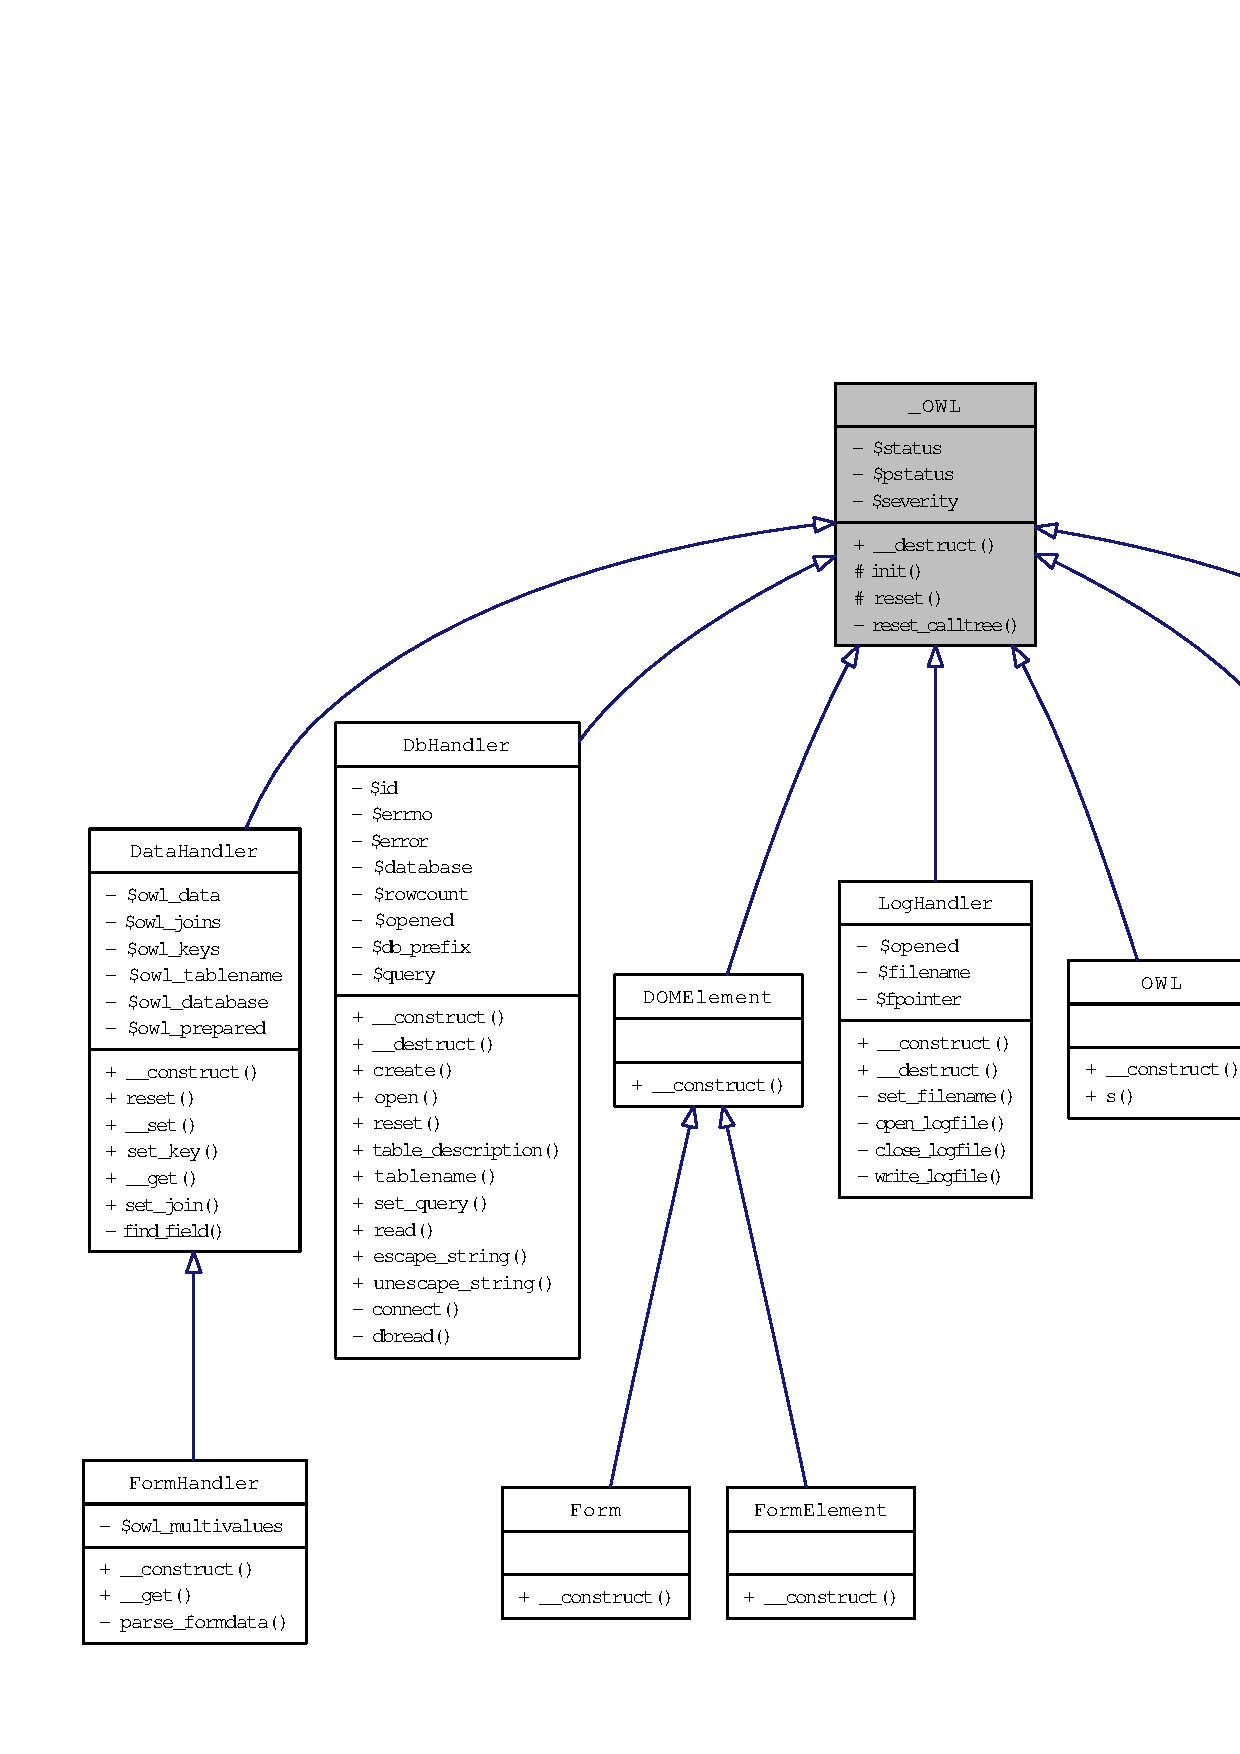
\includegraphics[height=400pt]{class__OWL__inherit__graph}
\end{center}
\end{figure}
\subsection*{Public Member Functions}
\begin{CompactItemize}
\item 
\hyperlink{class__OWL_99ec771fa2c5c279f80152cc09e489a8}{get\_\-status} ()
\item 
\hyperlink{class__OWL_61c04b80fe17e2f1e339a6d6a89e45f3}{signal} (\$level=0)
\end{CompactItemize}
\subsection*{Protected Member Functions}
\begin{CompactItemize}
\item 
\hyperlink{class__OWL_e0ef3ded56e8a6b34b6461e5a721cd3e}{init} ()
\item 
\hyperlink{class__OWL_5b88d497ccf2305fa411b9bd3f4bfe6f}{severity} ()
\item 
\hyperlink{class__OWL_2f2a042bcf31965194c03033df0edc9b}{reset} ()
\item 
\hyperlink{class__OWL_ea912d0ede9b3c2a69b79072d94d4787}{set\_\-status} (\$status, \$params=array())
\end{CompactItemize}
\subsection*{Protected Attributes}
\begin{CompactItemize}
\item 
\hyperlink{class__OWL_f37a011667dda12fc417a68a6f3077d1}{\$config}
\end{CompactItemize}
\subsection*{Private Attributes}
\begin{CompactItemize}
\item 
\hyperlink{class__OWL_af448f6bc8a90e20c09e9e2b8fe46eb5}{\$status}
\item 
\hyperlink{class__OWL_9cd573fffbb55aa42f29d83b39308528}{\$message\_\-params}
\end{CompactItemize}


\subsection{Detailed Description}
This is the main class for all OWL objects. It contains some methods that have to be available to all objects. Some of them can be reimplemented. \begin{Desc}
\item[Author:]Oscar van Eijk, Oveas Functionality Provider \end{Desc}
\begin{Desc}
\item[Version:]May 15, 2007 -- O van Eijk -- initial version \end{Desc}


\subsection{Member Function Documentation}
\hypertarget{class__OWL_e0ef3ded56e8a6b34b6461e5a721cd3e}{
\index{\_\-OWL@{\_\-OWL}!init@{init}}
\index{init@{init}!_OWL@{\_\-OWL}}
\subsubsection{\setlength{\rightskip}{0pt plus 5cm}\_\-OWL::init ()\hspace{0.3cm}{\tt  \mbox{[}protected\mbox{]}}}}
\label{class__OWL_e0ef3ded56e8a6b34b6461e5a721cd3e}


This function should be called by all constuctors. It initializes the general characteristics. Status is 'warning' by default, it's up to the contructor to set a proper status; if it's still 'warning', this $\ast$might$\ast$ indicate something went wrong. \hypertarget{class__OWL_5b88d497ccf2305fa411b9bd3f4bfe6f}{
\index{\_\-OWL@{\_\-OWL}!severity@{severity}}
\index{severity@{severity}!_OWL@{\_\-OWL}}
\subsubsection{\setlength{\rightskip}{0pt plus 5cm}\_\-OWL::severity ()\hspace{0.3cm}{\tt  \mbox{[}protected\mbox{]}}}}
\label{class__OWL_5b88d497ccf2305fa411b9bd3f4bfe6f}


Check the status of the given object and return its severity. \hypertarget{class__OWL_2f2a042bcf31965194c03033df0edc9b}{
\index{\_\-OWL@{\_\-OWL}!reset@{reset}}
\index{reset@{reset}!_OWL@{\_\-OWL}}
\subsubsection{\setlength{\rightskip}{0pt plus 5cm}\_\-OWL::reset ()\hspace{0.3cm}{\tt  \mbox{[}protected\mbox{]}}}}
\label{class__OWL_2f2a042bcf31965194c03033df0edc9b}


General reset function for all objects. Should be called after each non-fatal error 

Reimplemented in \hyperlink{classDbHandler_9982df4830f05803935bb31bac7fae3d}{DbHandler}.\hypertarget{class__OWL_ea912d0ede9b3c2a69b79072d94d4787}{
\index{\_\-OWL@{\_\-OWL}!set\_\-status@{set\_\-status}}
\index{set\_\-status@{set\_\-status}!_OWL@{\_\-OWL}}
\subsubsection{\setlength{\rightskip}{0pt plus 5cm}\_\-OWL::set\_\-status (\$ {\em status}, \$ {\em params} = {\tt array~()})\hspace{0.3cm}{\tt  \mbox{[}protected\mbox{]}}}}
\label{class__OWL_ea912d0ede9b3c2a69b79072d94d4787}


Set the current object status to the specified value.

\begin{Desc}
\item[Parameters:]
\begin{description}
\item[\mbox{$\leftarrow$} {\em \$status}]OWL status code \item[\mbox{$\leftarrow$} {\em \$params}]\end{description}
\end{Desc}
\hypertarget{class__OWL_99ec771fa2c5c279f80152cc09e489a8}{
\index{\_\-OWL@{\_\-OWL}!get\_\-status@{get\_\-status}}
\index{get\_\-status@{get\_\-status}!_OWL@{\_\-OWL}}
\subsubsection{\setlength{\rightskip}{0pt plus 5cm}\_\-OWL::get\_\-status ()}}
\label{class__OWL_99ec771fa2c5c279f80152cc09e489a8}


Get the current object status.

\begin{Desc}
\item[Returns:]Object's status code \end{Desc}
\hypertarget{class__OWL_61c04b80fe17e2f1e339a6d6a89e45f3}{
\index{\_\-OWL@{\_\-OWL}!signal@{signal}}
\index{signal@{signal}!_OWL@{\_\-OWL}}
\subsubsection{\setlength{\rightskip}{0pt plus 5cm}\_\-OWL::signal (\$ {\em level} = {\tt 0})}}
\label{class__OWL_61c04b80fe17e2f1e339a6d6a89e45f3}


Display the message for the current object status

\begin{Desc}
\item[Parameters:]
\begin{description}
\item[\mbox{$\leftarrow$} {\em \$level}]An optional severity level; message will only be displayed when it is at least of this level. \end{description}
\end{Desc}
\begin{Desc}
\item[Returns:]The severity level for this object \end{Desc}


\subsection{Member Data Documentation}
\hypertarget{class__OWL_af448f6bc8a90e20c09e9e2b8fe46eb5}{
\index{\_\-OWL@{\_\-OWL}!\$status@{\$status}}
\index{\$status@{\$status}!_OWL@{\_\-OWL}}
\subsubsection{\setlength{\rightskip}{0pt plus 5cm}\_\-OWL::\$status\hspace{0.3cm}{\tt  \mbox{[}private\mbox{]}}}}
\label{class__OWL_af448f6bc8a90e20c09e9e2b8fe46eb5}


Current object status \hypertarget{class__OWL_9cd573fffbb55aa42f29d83b39308528}{
\index{\_\-OWL@{\_\-OWL}!\$message\_\-params@{\$message\_\-params}}
\index{\$message\_\-params@{\$message\_\-params}!_OWL@{\_\-OWL}}
\subsubsection{\setlength{\rightskip}{0pt plus 5cm}\_\-OWL::\$message\_\-params\hspace{0.3cm}{\tt  \mbox{[}private\mbox{]}}}}
\label{class__OWL_9cd573fffbb55aa42f29d83b39308528}


Array with parameters that will be substituted in message text \hypertarget{class__OWL_f37a011667dda12fc417a68a6f3077d1}{
\index{\_\-OWL@{\_\-OWL}!\$config@{\$config}}
\index{\$config@{\$config}!_OWL@{\_\-OWL}}
\subsubsection{\setlength{\rightskip}{0pt plus 5cm}\_\-OWL::\$config\hspace{0.3cm}{\tt  \mbox{[}protected\mbox{]}}}}
\label{class__OWL_f37a011667dda12fc417a68a6f3077d1}


The global Config array is referenced from every object 

The documentation for this class was generated from the following file:\begin{CompactItemize}
\item 
/home/oscar/work/eclipse/owl-php/src/inc/\hyperlink{class_8__OWL_8php}{class.\_\-OWL.php}\end{CompactItemize}

\hypertarget{classDataHandler}{
\section{DataHandler Class Reference}
\label{classDataHandler}\index{DataHandler@{DataHandler}}
}
The OWL Data object.  


Inheritance diagram for DataHandler:\nopagebreak
\begin{figure}[H]
\begin{center}
\leavevmode
\includegraphics[height=400pt]{classDataHandler__inherit__graph}
\end{center}
\end{figure}
Collaboration diagram for DataHandler:\nopagebreak
\begin{figure}[H]
\begin{center}
\leavevmode
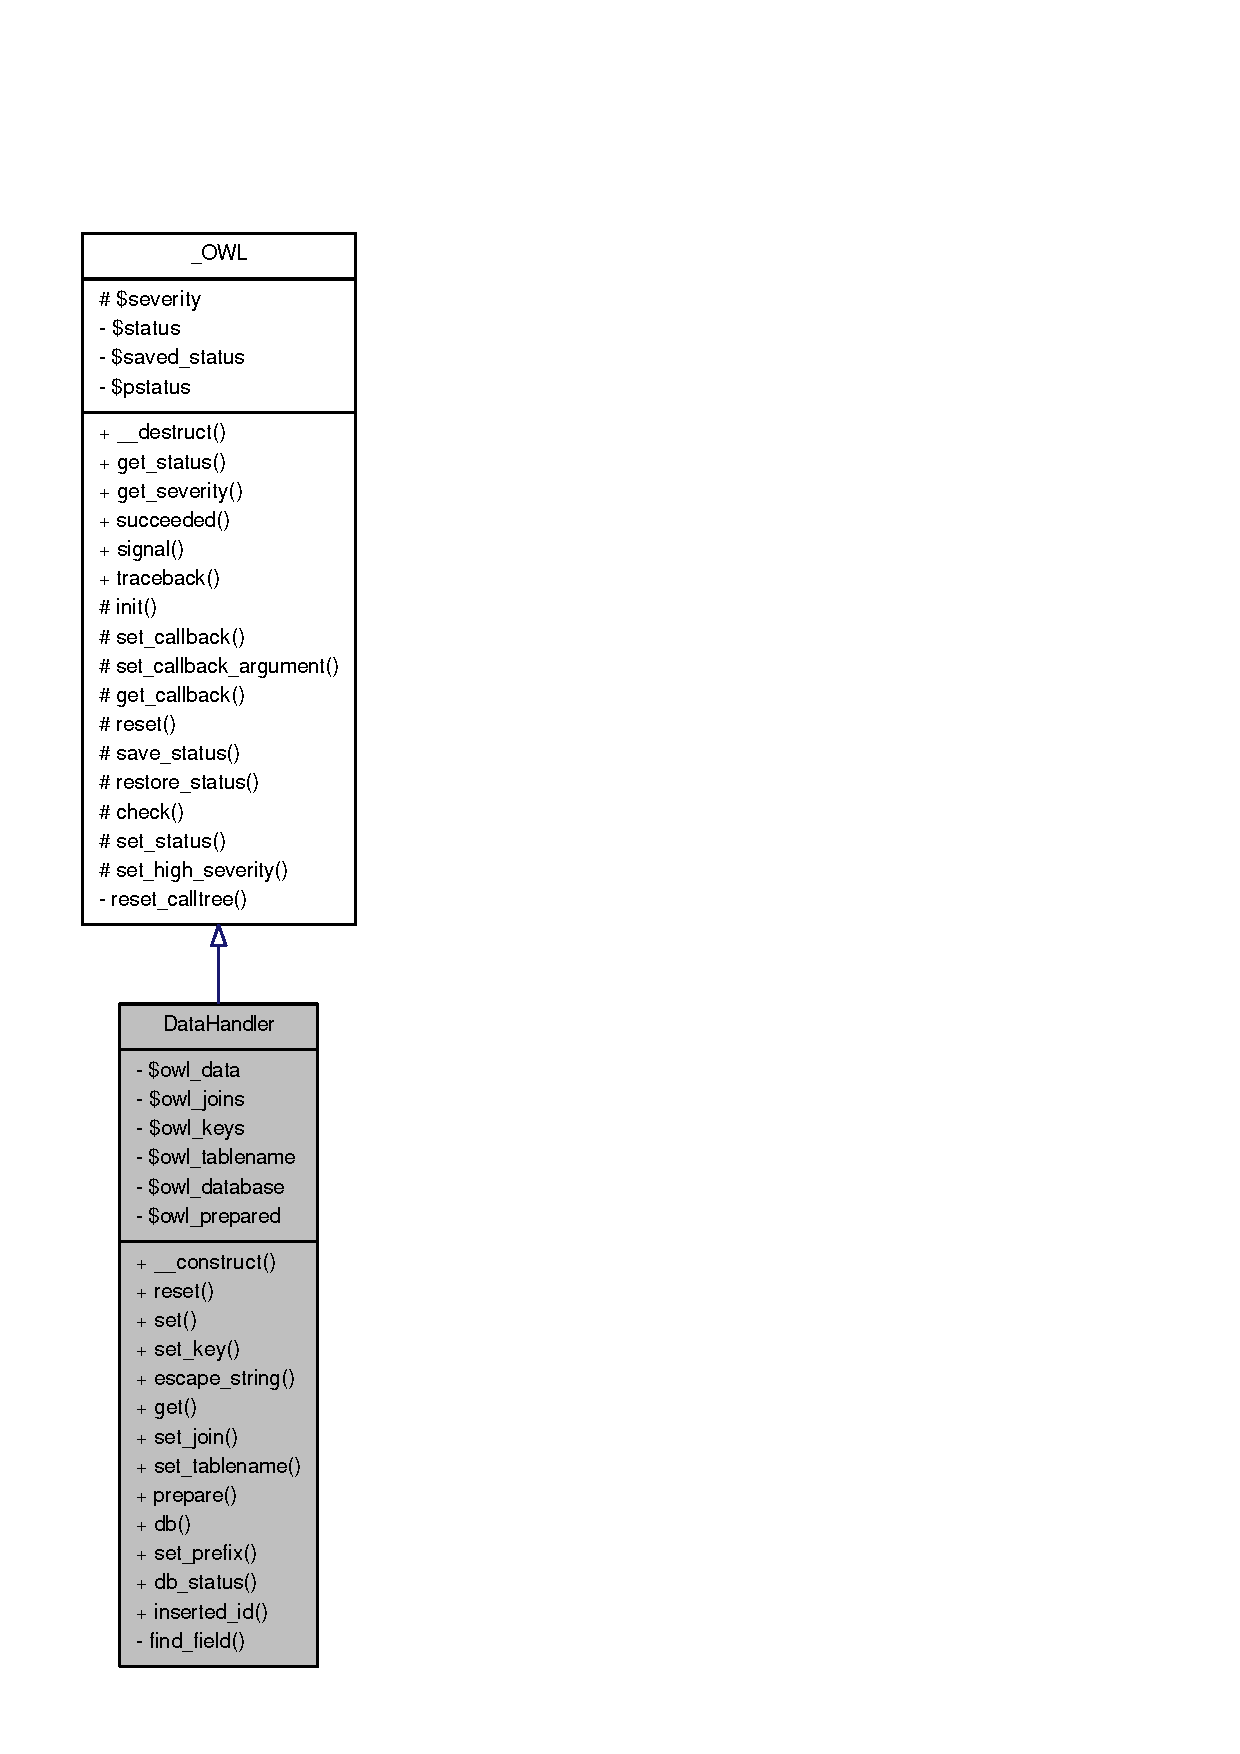
\includegraphics[height=400pt]{classDataHandler__coll__graph}
\end{center}
\end{figure}
\subsection*{Public Member Functions}
\begin{CompactItemize}
\item 
\hyperlink{classDataHandler_4eef16167dd9a5bc94bd0cb40ce1b180}{\_\-\_\-construct} (\$dblink=null, \$tablename= '')
\item 
\hyperlink{classDataHandler_b89e1aaad9cd0a37f1c7f13c1d9c0d57}{reset} (\$level=\hyperlink{class_8datahandler_8php_19a99423705b41e563424ae76d7fe184}{DATA\_\-RESET\_\-PREPARE})
\item 
\hyperlink{classDataHandler_16c81c9564a7feaf530ce5d51ed99df7}{\_\-\_\-set} (\$variable, \$value)
\item 
\hyperlink{classDataHandler_32ce223478b78a4ea9838a3c6ac7440c}{set\_\-key} (\$variable)
\item 
\hyperlink{classDataHandler_f58cbd10b032e4904fa15ce950d521e2}{\_\-\_\-get} (\$variable)
\item 
\hyperlink{classDataHandler_9b77733f02e9d6281fc40df110c0ba70}{set\_\-join} (\$lvalue, \$rvalue, \$linktype= '=')
\end{CompactItemize}
\subsection*{Protected Member Functions}
\begin{CompactItemize}
\item 
\hyperlink{class__OWL_e0ef3ded56e8a6b34b6461e5a721cd3e}{init} ()
\item 
\hyperlink{class__OWL_2f2a042bcf31965194c03033df0edc9b}{reset} ()
\end{CompactItemize}
\subsection*{Protected Attributes}
\begin{CompactItemize}
\item 
\hyperlink{class__OWL_f37a011667dda12fc417a68a6f3077d1}{\$config}
\end{CompactItemize}
\subsection*{Private Member Functions}
\begin{CompactItemize}
\item 
\hyperlink{classDataHandler_1e4789e22370c96ae479bc3a58f30984}{find\_\-field} (\$fld, \&\$expanded)
\end{CompactItemize}
\subsection*{Private Attributes}
\begin{CompactItemize}
\item 
\hyperlink{classDataHandler_329b5524c379e0db6c4d5ce59f3c414f}{\$owl\_\-data}
\item 
\hyperlink{classDataHandler_da9b697f81ea82d269077f9c7445791d}{\$owl\_\-joins}
\item 
\hyperlink{classDataHandler_8d398720bce975159b2d13ad7a941bc7}{\$owl\_\-keys}
\item 
\hyperlink{classDataHandler_24620784bde262bdd02227962d3b9605}{\$owl\_\-tablename}
\item 
\hyperlink{classDataHandler_3ac49aa018e0ebe4c74f5a636d455a8b}{\$owl\_\-database}
\item 
\hyperlink{classDataHandler_e6093d21291ed3ab3183e11962452928}{\$owl\_\-prepared}
\end{CompactItemize}


\subsection{Detailed Description}
The OWL Data object. 

This class contains DB datasets \begin{Desc}
\item[Author:]Oscar van Eijk, Oveas Functionality Provider \end{Desc}
\begin{Desc}
\item[Version:]Aug 4, 2008 -- O van Eijk -- initial version \end{Desc}


\subsection{Constructor \& Destructor Documentation}
\hypertarget{classDataHandler_4eef16167dd9a5bc94bd0cb40ce1b180}{
\index{DataHandler@{DataHandler}!\_\-\_\-construct@{\_\-\_\-construct}}
\index{\_\-\_\-construct@{\_\-\_\-construct}!DataHandler@{DataHandler}}
\subsubsection{\setlength{\rightskip}{0pt plus 5cm}DataHandler::\_\-\_\-construct (\$ {\em dblink} = {\tt null}, \$ {\em tablename} = {\tt ''})}}
\label{classDataHandler_4eef16167dd9a5bc94bd0cb40ce1b180}


Class constructor \begin{Desc}
\item[Parameters:]
\begin{description}
\item[\mbox{$\leftarrow$} {\em \$dblink}]Database object \item[\mbox{$\leftarrow$} {\em \$tablename}]Default table name for this dataset \end{description}
\end{Desc}


\subsection{Member Function Documentation}
\hypertarget{classDataHandler_b89e1aaad9cd0a37f1c7f13c1d9c0d57}{
\index{DataHandler@{DataHandler}!reset@{reset}}
\index{reset@{reset}!DataHandler@{DataHandler}}
\subsubsection{\setlength{\rightskip}{0pt plus 5cm}DataHandler::reset (\$ {\em level} = {\tt {\bf DATA\_\-RESET\_\-PREPARE}})}}
\label{classDataHandler_b89e1aaad9cd0a37f1c7f13c1d9c0d57}


Reset the object \begin{Desc}
\item[Parameters:]
\begin{description}
\item[\mbox{$\leftarrow$} {\em \$level}]The reset level, can be any of the following:\begin{itemize}
\item DATA\_\-RESET\_\-STATUS; Reset object status only\item DATA\_\-RESET\_\-PREPARE (default); Reset status and a prepared query\item DATA\_\-RESET\_\-META; Reset status and query, remove all locks and joins\item DATA\_\-RESET\_\-FULL; Reset status and query, remove all locks, joins and data \end{itemize}
\end{description}
\end{Desc}
\hypertarget{classDataHandler_16c81c9564a7feaf530ce5d51ed99df7}{
\index{DataHandler@{DataHandler}!\_\-\_\-set@{\_\-\_\-set}}
\index{\_\-\_\-set@{\_\-\_\-set}!DataHandler@{DataHandler}}
\subsubsection{\setlength{\rightskip}{0pt plus 5cm}DataHandler::\_\-\_\-set (\$ {\em variable}, \$ {\em value})}}
\label{classDataHandler_16c81c9564a7feaf530ce5d51ed99df7}


Define or override a variable in the data array

\begin{Desc}
\item[Parameters:]
\begin{description}
\item[\mbox{$\leftarrow$} {\em \$variable}]The name of the variable that should be set \item[\mbox{$\leftarrow$} {\em \$value}]Value to set the variable to. If this is an array, the second field in the array has to be the tablename where the fieldname is found. The value itself van NEVER be an array! \end{description}
\end{Desc}
\hypertarget{classDataHandler_32ce223478b78a4ea9838a3c6ac7440c}{
\index{DataHandler@{DataHandler}!set\_\-key@{set\_\-key}}
\index{set\_\-key@{set\_\-key}!DataHandler@{DataHandler}}
\subsubsection{\setlength{\rightskip}{0pt plus 5cm}DataHandler::set\_\-key (\$ {\em variable})}}
\label{classDataHandler_32ce223478b78a4ea9838a3c6ac7440c}


Lock variables for update by adding them to an array. Fields in this array will not be overwritten on updates, but used in WHERE clauses. \begin{Desc}
\item[Parameters:]
\begin{description}
\item[\mbox{$\leftarrow$} {\em \$variable}]Variable name to lock, optionally as an array (table, field) \end{description}
\end{Desc}
\begin{Desc}
\item[Returns:]Severity level \end{Desc}
\hypertarget{classDataHandler_1e4789e22370c96ae479bc3a58f30984}{
\index{DataHandler@{DataHandler}!find\_\-field@{find\_\-field}}
\index{find\_\-field@{find\_\-field}!DataHandler@{DataHandler}}
\subsubsection{\setlength{\rightskip}{0pt plus 5cm}DataHandler::find\_\-field (\$ {\em fld}, \&\$ {\em expanded})\hspace{0.3cm}{\tt  \mbox{[}private\mbox{]}}}}
\label{classDataHandler_1e4789e22370c96ae479bc3a58f30984}


Try to exand a field to a fully qualified 'table\#field' name

\begin{Desc}
\item[Parameters:]
\begin{description}
\item[\mbox{$\leftarrow$} {\em \$fld}]The fieldname that has to be expanded \item[\mbox{$\rightarrow$} {\em \$expanded}]An array with all matching fully qualified fieldnames. \end{description}
\end{Desc}
\begin{Desc}
\item[Returns:]The number of matches \end{Desc}
\hypertarget{classDataHandler_f58cbd10b032e4904fa15ce950d521e2}{
\index{DataHandler@{DataHandler}!\_\-\_\-get@{\_\-\_\-get}}
\index{\_\-\_\-get@{\_\-\_\-get}!DataHandler@{DataHandler}}
\subsubsection{\setlength{\rightskip}{0pt plus 5cm}DataHandler::\_\-\_\-get (\$ {\em variable})}}
\label{classDataHandler_f58cbd10b032e4904fa15ce950d521e2}


Retrieve a value from the data array. The variable name can be a fully qualified table/fieldname (format \char`\"{}table\#field\char`\"{}), or only a field name, in which case it has to be unique. If the fieldname cannot be found directly, the array is scanned to find a matching field. It more matches are found, the object status is set to DATA\_\-AMBFIELD.

\begin{Desc}
\item[Parameters:]
\begin{description}
\item[\mbox{$\leftarrow$} {\em \$variable}]The name of the variable that should be retrieved \end{description}
\end{Desc}
\begin{Desc}
\item[Returns:]The value, or NULL when the value was not found or abigious. \end{Desc}
\hypertarget{classDataHandler_9b77733f02e9d6281fc40df110c0ba70}{
\index{DataHandler@{DataHandler}!set\_\-join@{set\_\-join}}
\index{set\_\-join@{set\_\-join}!DataHandler@{DataHandler}}
\subsubsection{\setlength{\rightskip}{0pt plus 5cm}DataHandler::set\_\-join (\$ {\em lvalue}, \$ {\em rvalue}, \$ {\em linktype} = {\tt '='})}}
\label{classDataHandler_9b77733f02e9d6281fc40df110c0ba70}


Define a link between 2 fields that will be recognized when the database query is built.

\begin{Desc}
\item[Parameters:]
\begin{description}
\item[\mbox{$\leftarrow$} {\em \$lvalue}]Left value as array(table, field) \item[\mbox{$\leftarrow$} {\em \$rvalue}]Right value as array(table, field) \item[\mbox{$\leftarrow$} {\em \$linktype}]How are the fields linked. Can be any binary operator as recognized by SQL. \end{description}
\end{Desc}
\begin{Desc}
\item[Returns:]Severity level \end{Desc}
\hypertarget{class__OWL_e0ef3ded56e8a6b34b6461e5a721cd3e}{
\index{DataHandler@{DataHandler}!init@{init}}
\index{init@{init}!DataHandler@{DataHandler}}
\subsubsection{\setlength{\rightskip}{0pt plus 5cm}\_\-OWL::init ()\hspace{0.3cm}{\tt  \mbox{[}final, protected, inherited\mbox{]}}}}
\label{class__OWL_e0ef3ded56e8a6b34b6461e5a721cd3e}


This function should be called by all constuctors. It initializes the general characteristics. Status is 'warning' by default, it's up to the contructor to set a proper status; if it's still 'warning', this $\ast$might$\ast$ indicate something went wrong. \hypertarget{class__OWL_2f2a042bcf31965194c03033df0edc9b}{
\index{DataHandler@{DataHandler}!reset@{reset}}
\index{reset@{reset}!DataHandler@{DataHandler}}
\subsubsection{\setlength{\rightskip}{0pt plus 5cm}\_\-OWL::reset ()\hspace{0.3cm}{\tt  \mbox{[}protected, inherited\mbox{]}}}}
\label{class__OWL_2f2a042bcf31965194c03033df0edc9b}


General reset function for all objects. Should be called after each non-fatal error 

Reimplemented in \hyperlink{classDbHandler_9982df4830f05803935bb31bac7fae3d}{DbHandler}.

\subsection{Member Data Documentation}
\hypertarget{classDataHandler_329b5524c379e0db6c4d5ce59f3c414f}{
\index{DataHandler@{DataHandler}!\$owl\_\-data@{\$owl\_\-data}}
\index{\$owl\_\-data@{\$owl\_\-data}!DataHandler@{DataHandler}}
\subsubsection{\setlength{\rightskip}{0pt plus 5cm}DataHandler::\$owl\_\-data\hspace{0.3cm}{\tt  \mbox{[}private\mbox{]}}}}
\label{classDataHandler_329b5524c379e0db6c4d5ce59f3c414f}


Indexed array holding all data values. \hypertarget{classDataHandler_da9b697f81ea82d269077f9c7445791d}{
\index{DataHandler@{DataHandler}!\$owl\_\-joins@{\$owl\_\-joins}}
\index{\$owl\_\-joins@{\$owl\_\-joins}!DataHandler@{DataHandler}}
\subsubsection{\setlength{\rightskip}{0pt plus 5cm}DataHandler::\$owl\_\-joins\hspace{0.3cm}{\tt  \mbox{[}private\mbox{]}}}}
\label{classDataHandler_da9b697f81ea82d269077f9c7445791d}


2D Array holding all relationships between the data. \hypertarget{classDataHandler_8d398720bce975159b2d13ad7a941bc7}{
\index{DataHandler@{DataHandler}!\$owl\_\-keys@{\$owl\_\-keys}}
\index{\$owl\_\-keys@{\$owl\_\-keys}!DataHandler@{DataHandler}}
\subsubsection{\setlength{\rightskip}{0pt plus 5cm}DataHandler::\$owl\_\-keys\hspace{0.3cm}{\tt  \mbox{[}private\mbox{]}}}}
\label{classDataHandler_8d398720bce975159b2d13ad7a941bc7}


Array with variable names that are used in WHERE clauses on updates \hypertarget{classDataHandler_24620784bde262bdd02227962d3b9605}{
\index{DataHandler@{DataHandler}!\$owl\_\-tablename@{\$owl\_\-tablename}}
\index{\$owl\_\-tablename@{\$owl\_\-tablename}!DataHandler@{DataHandler}}
\subsubsection{\setlength{\rightskip}{0pt plus 5cm}DataHandler::\$owl\_\-tablename\hspace{0.3cm}{\tt  \mbox{[}private\mbox{]}}}}
\label{classDataHandler_24620784bde262bdd02227962d3b9605}


All variable names are expected to be fields in a database as well. If a table name is not given, the default table name will be used. This is useful for datasets that come from only one database table. For datasets that are not read from or written to a database, the tablename can be null. \hypertarget{classDataHandler_3ac49aa018e0ebe4c74f5a636d455a8b}{
\index{DataHandler@{DataHandler}!\$owl\_\-database@{\$owl\_\-database}}
\index{\$owl\_\-database@{\$owl\_\-database}!DataHandler@{DataHandler}}
\subsubsection{\setlength{\rightskip}{0pt plus 5cm}DataHandler::\$owl\_\-database\hspace{0.3cm}{\tt  \mbox{[}private\mbox{]}}}}
\label{classDataHandler_3ac49aa018e0ebe4c74f5a636d455a8b}


An optional link to a database object. This has to be specified if the data needs to be written to or read from a dabatase. \hypertarget{classDataHandler_e6093d21291ed3ab3183e11962452928}{
\index{DataHandler@{DataHandler}!\$owl\_\-prepared@{\$owl\_\-prepared}}
\index{\$owl\_\-prepared@{\$owl\_\-prepared}!DataHandler@{DataHandler}}
\subsubsection{\setlength{\rightskip}{0pt plus 5cm}DataHandler::\$owl\_\-prepared\hspace{0.3cm}{\tt  \mbox{[}private\mbox{]}}}}
\label{classDataHandler_e6093d21291ed3ab3183e11962452928}


Boolean that indicates of a query has been prepared \hypertarget{class__OWL_f37a011667dda12fc417a68a6f3077d1}{
\index{DataHandler@{DataHandler}!\$config@{\$config}}
\index{\$config@{\$config}!DataHandler@{DataHandler}}
\subsubsection{\setlength{\rightskip}{0pt plus 5cm}\_\-OWL::\$config\hspace{0.3cm}{\tt  \mbox{[}protected, inherited\mbox{]}}}}
\label{class__OWL_f37a011667dda12fc417a68a6f3077d1}


The global Config array is referenced from every object 

The documentation for this class was generated from the following file:\begin{CompactItemize}
\item 
/home/oscar/work/eclipse/owl-php/src/inc/\hyperlink{class_8datahandler_8php}{class.datahandler.php}\end{CompactItemize}

\hypertarget{classDbHandler}{
\section{DbHandler Class Reference}
\label{classDbHandler}\index{DbHandler@{DbHandler}}
}
Database handler.  


Inheritance diagram for DbHandler:\nopagebreak
\begin{figure}[H]
\begin{center}
\leavevmode
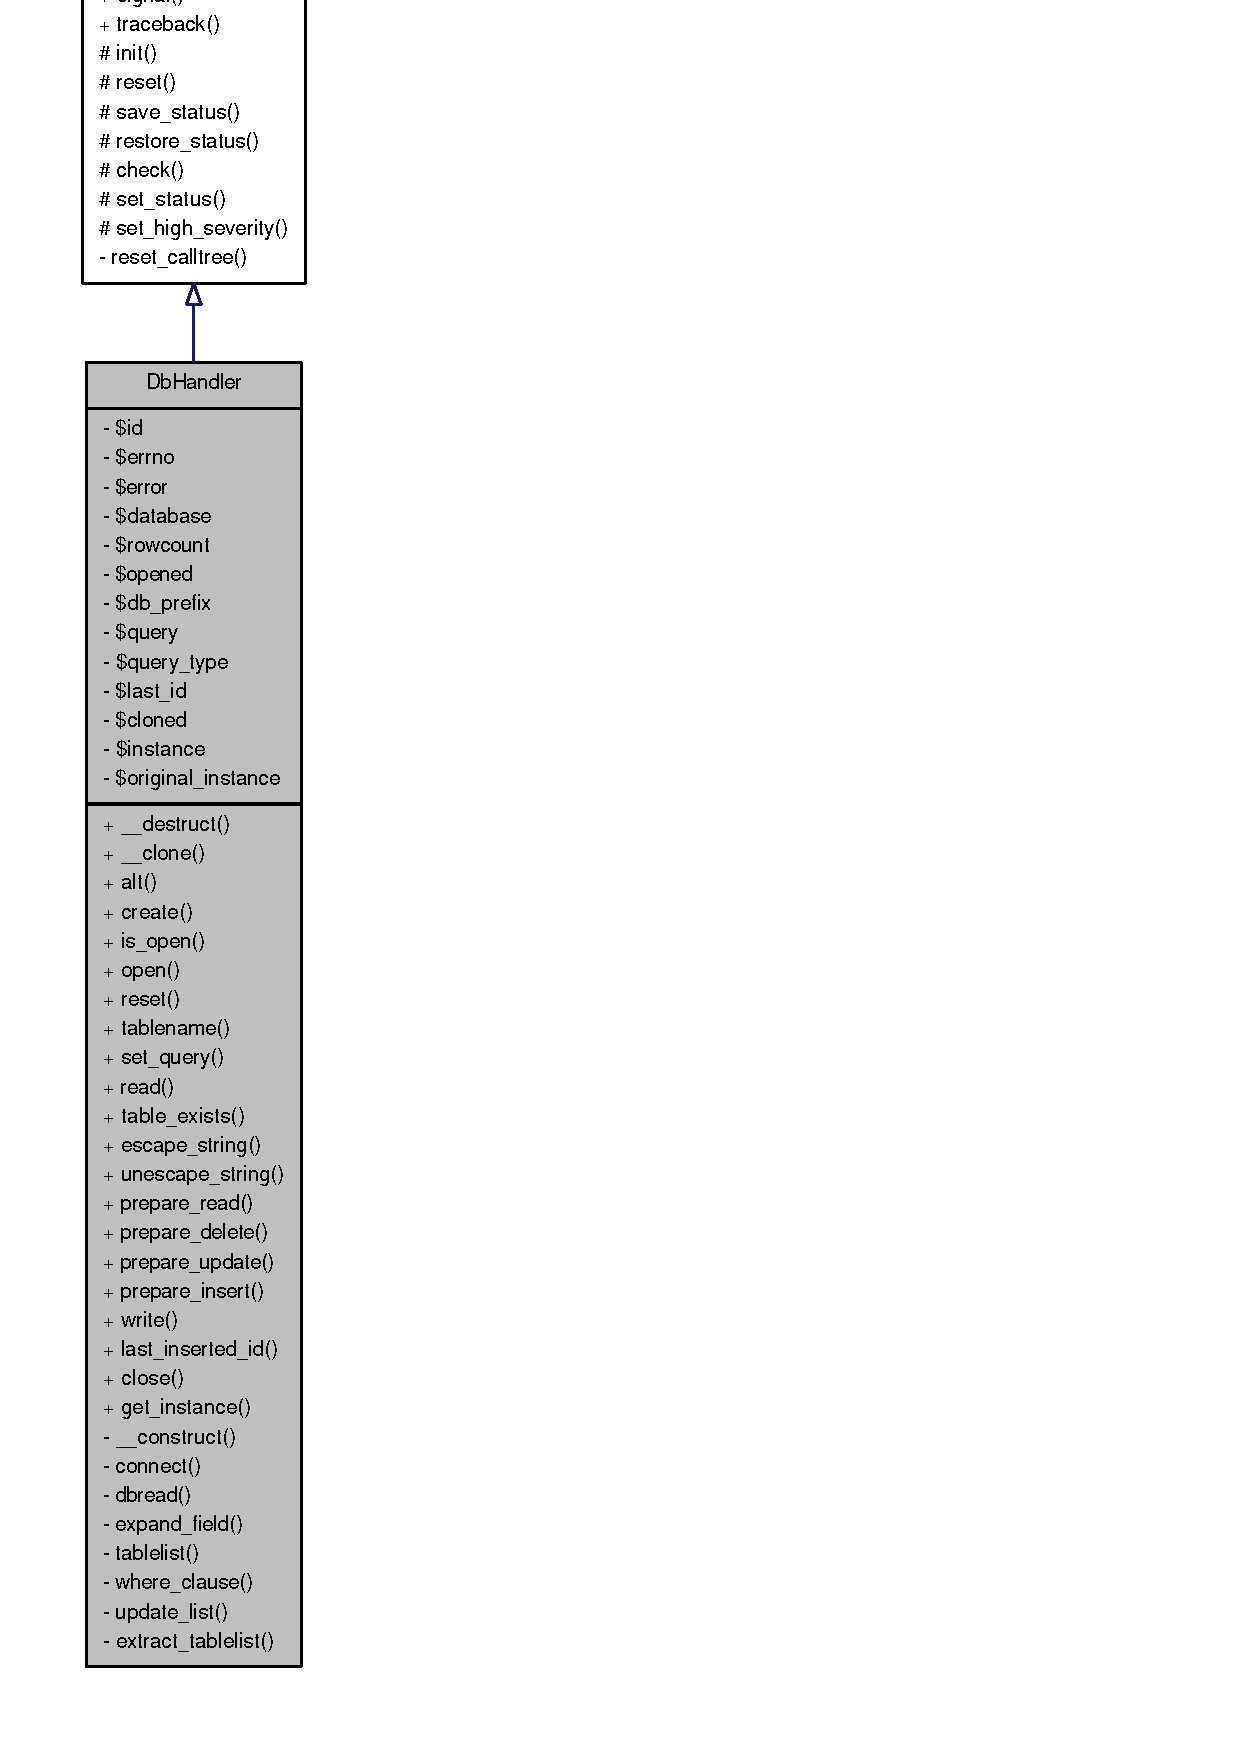
\includegraphics[height=400pt]{classDbHandler__inherit__graph}
\end{center}
\end{figure}
Collaboration diagram for DbHandler:\nopagebreak
\begin{figure}[H]
\begin{center}
\leavevmode
\includegraphics[height=400pt]{classDbHandler__coll__graph}
\end{center}
\end{figure}
\subsection*{Public Member Functions}
\begin{CompactItemize}
\item 
\hyperlink{classDbHandler_e54e9d4643f41a9296167086f6a769fc}{\_\-\_\-construct} (\$srv= 'localhost', \$db= '', \$usr= '', \$pwd= '', \$dbtype= 'MySQL')
\item 
\hyperlink{classDbHandler_7cd6bd727d1f296eb5dbfae6ca36ab3f}{\_\-\_\-destruct} ()
\item 
\hyperlink{classDbHandler_c9e93cb0ab57f03b2719eebd0c0ee2ef}{create} ()
\item 
\hyperlink{classDbHandler_fccbfc69ead84f8445116e050d1cfc2d}{open} ()
\item 
\hyperlink{classDbHandler_9982df4830f05803935bb31bac7fae3d}{reset} ()
\item 
\hyperlink{classDbHandler_00402b0e3e677108716714fbf94bea40}{table\_\-description} (\$tablename, \&\$data)
\item 
\hyperlink{classDbHandler_baca15a312800e5522b3efd9dff036f5}{tablename} (\$tablename)
\item 
\hyperlink{classDbHandler_305a3225c4760a88a06b0d55d0893962}{set\_\-query} (\$qry)
\item 
\hyperlink{classDbHandler_5ebfdc2acfcb0e9cbc2861fc55c7127c}{read} (\$flag=\hyperlink{class_8dbhandler_8php_cc5178c2a582eafa4ef488ed3394b725}{DBHANDLE\_\-DATA}, \&\$data, \$quick\_\-query= '', \$line=0, \$file= '\mbox{[}unknown\mbox{]}')
\item 
\hyperlink{classDbHandler_67d77702ff6db70f89123d3f947af143}{escape\_\-string} (\$string)
\item 
\hyperlink{classDbHandler_27c604b14c39913d34630e5504979b15}{unescape\_\-string} (\$string)
\end{CompactItemize}
\subsection*{Protected Member Functions}
\begin{CompactItemize}
\item 
\hyperlink{class__OWL_e0ef3ded56e8a6b34b6461e5a721cd3e}{init} ()
\end{CompactItemize}
\subsection*{Private Member Functions}
\begin{CompactItemize}
\item 
\hyperlink{classDbHandler_9cf52ba614981a0082063d57290d3b7c}{connect} ()
\item 
\hyperlink{classDbHandler_130e49aa639fecb46ce6719ddcb0d72f}{dbread} (\$qry, \&\$rows, \&\$fields)
\end{CompactItemize}
\subsection*{Private Attributes}
\begin{CompactItemize}
\item 
\hyperlink{classDbHandler_d38e1c3312815c8ad4093957881092ff}{\$id}
\item 
\hyperlink{classDbHandler_f6e9f493be56617cb533763bb2a0e85a}{\$errno}
\item 
\hyperlink{classDbHandler_de79e11156abbfc180864beb5b9df377}{\$error}
\item 
\hyperlink{classDbHandler_faac5248f9ee59786b48a7b51f318940}{\$database}
\item 
\hyperlink{classDbHandler_56a7ae4bd7d842c85f3fe8052aecbfef}{\$rowcount}
\item 
\hyperlink{classDbHandler_71e36ffbff0d157b1d91dc000bc6f821}{\$opened}
\item 
\hyperlink{classDbHandler_19af96598e7f72673fc5da26ad77731b}{\$db\_\-prefix}
\item 
\hyperlink{classDbHandler_d671b5596b37dac6d48a660a07775965}{\$query}
\end{CompactItemize}


\subsection{Detailed Description}
Database handler. 

Handler for all database I/O. This class uses an (abstract) class for the actual storage. \begin{Desc}
\item[Author:]Oscar van Eijk, Oveas Functionality Provider \end{Desc}
\begin{Desc}
\item[Version:]May 15, 2007 -- O van Eijk -- initial version for Terra-Terra 

Jul 29, 2008 -- O van Eijk -- Modified version for \hyperlink{classOWL}{OWL} \end{Desc}


\subsection{Constructor \& Destructor Documentation}
\hypertarget{classDbHandler_e54e9d4643f41a9296167086f6a769fc}{
\index{DbHandler@{DbHandler}!\_\-\_\-construct@{\_\-\_\-construct}}
\index{\_\-\_\-construct@{\_\-\_\-construct}!DbHandler@{DbHandler}}
\subsubsection{\setlength{\rightskip}{0pt plus 5cm}DbHandler::\_\-\_\-construct (\$ {\em srv} = {\tt 'localhost'}, \$ {\em db} = {\tt ''}, \$ {\em usr} = {\tt ''}, \$ {\em pwd} = {\tt ''}, \$ {\em dbtype} = {\tt 'MySQL'})}}
\label{classDbHandler_e54e9d4643f41a9296167086f6a769fc}


Class constructor; opens the database connection.

\begin{Desc}
\item[Parameters:]
\begin{description}
\item[\mbox{$\leftarrow$} {\em \$srv}]Database server \item[\mbox{$\leftarrow$} {\em \$db}]Database name \item[\mbox{$\leftarrow$} {\em \$usr}]Username to connect with \item[\mbox{$\leftarrow$} {\em \$pwd}]Password to use for connection \item[\mbox{$\leftarrow$} {\em \$dbtype}]Database type (reserved for future use, currently only MySQL is implemented) \end{description}
\end{Desc}
\hypertarget{classDbHandler_7cd6bd727d1f296eb5dbfae6ca36ab3f}{
\index{DbHandler@{DbHandler}!\_\-\_\-destruct@{\_\-\_\-destruct}}
\index{\_\-\_\-destruct@{\_\-\_\-destruct}!DbHandler@{DbHandler}}
\subsubsection{\setlength{\rightskip}{0pt plus 5cm}DbHandler::\_\-\_\-destruct ()}}
\label{classDbHandler_7cd6bd727d1f296eb5dbfae6ca36ab3f}


Class destructor; closes the database connection 

Reimplemented from \hyperlink{class__OWL_44fd2222476a3109286cc82d92b6bbcc}{\_\-OWL}.

\subsection{Member Function Documentation}
\hypertarget{classDbHandler_c9e93cb0ab57f03b2719eebd0c0ee2ef}{
\index{DbHandler@{DbHandler}!create@{create}}
\index{create@{create}!DbHandler@{DbHandler}}
\subsubsection{\setlength{\rightskip}{0pt plus 5cm}DbHandler::create ()}}
\label{classDbHandler_c9e93cb0ab57f03b2719eebd0c0ee2ef}


Create a new database

\begin{Desc}
\item[Returns:]Severity level \end{Desc}
\hypertarget{classDbHandler_9cf52ba614981a0082063d57290d3b7c}{
\index{DbHandler@{DbHandler}!connect@{connect}}
\index{connect@{connect}!DbHandler@{DbHandler}}
\subsubsection{\setlength{\rightskip}{0pt plus 5cm}DbHandler::connect ()\hspace{0.3cm}{\tt  \mbox{[}private\mbox{]}}}}
\label{classDbHandler_9cf52ba614981a0082063d57290d3b7c}


Connect to the database server

\begin{Desc}
\item[Returns:]True on success, otherwise False \end{Desc}
\hypertarget{classDbHandler_fccbfc69ead84f8445116e050d1cfc2d}{
\index{DbHandler@{DbHandler}!open@{open}}
\index{open@{open}!DbHandler@{DbHandler}}
\subsubsection{\setlength{\rightskip}{0pt plus 5cm}DbHandler::open ()}}
\label{classDbHandler_fccbfc69ead84f8445116e050d1cfc2d}


Opens the database connection.

\begin{Desc}
\item[Returns:]Severity level \end{Desc}
\hypertarget{classDbHandler_9982df4830f05803935bb31bac7fae3d}{
\index{DbHandler@{DbHandler}!reset@{reset}}
\index{reset@{reset}!DbHandler@{DbHandler}}
\subsubsection{\setlength{\rightskip}{0pt plus 5cm}DbHandler::reset ()}}
\label{classDbHandler_9982df4830f05803935bb31bac7fae3d}


Reset the object 

Reimplemented from \hyperlink{class__OWL_2f2a042bcf31965194c03033df0edc9b}{\_\-OWL}.\hypertarget{classDbHandler_00402b0e3e677108716714fbf94bea40}{
\index{DbHandler@{DbHandler}!table\_\-description@{table\_\-description}}
\index{table\_\-description@{table\_\-description}!DbHandler@{DbHandler}}
\subsubsection{\setlength{\rightskip}{0pt plus 5cm}DbHandler::table\_\-description (\$ {\em tablename}, \&\$ {\em data})}}
\label{classDbHandler_00402b0e3e677108716714fbf94bea40}


Get a description of a database table

\begin{Desc}
\item[Parameters:]
\begin{description}
\item[\mbox{$\leftarrow$} {\em \$tablename}]The tablename \item[\mbox{$\rightarrow$} {\em \$data}]Indexed array holding all fields =$>$ datatypes \end{description}
\end{Desc}
\begin{Desc}
\item[Returns:]Indexed array holding all fields =$>$ datatypes \end{Desc}
\hypertarget{classDbHandler_baca15a312800e5522b3efd9dff036f5}{
\index{DbHandler@{DbHandler}!tablename@{tablename}}
\index{tablename@{tablename}!DbHandler@{DbHandler}}
\subsubsection{\setlength{\rightskip}{0pt plus 5cm}DbHandler::tablename (\$ {\em tablename})}}
\label{classDbHandler_baca15a312800e5522b3efd9dff036f5}


Extend a tablename with the database prefix

\begin{Desc}
\item[Parameters:]
\begin{description}
\item[\mbox{$\leftarrow$} {\em \$tablename}]Table name to extend \end{description}
\end{Desc}
\begin{Desc}
\item[Returns:]Extended table name \end{Desc}
\hypertarget{classDbHandler_305a3225c4760a88a06b0d55d0893962}{
\index{DbHandler@{DbHandler}!set\_\-query@{set\_\-query}}
\index{set\_\-query@{set\_\-query}!DbHandler@{DbHandler}}
\subsubsection{\setlength{\rightskip}{0pt plus 5cm}DbHandler::set\_\-query (\$ {\em qry})}}
\label{classDbHandler_305a3225c4760a88a06b0d55d0893962}


Set the database query. This function should only be used if the query is too complex to be set with any of the prepare() functions.

\begin{Desc}
\item[Parameters:]
\begin{description}
\item[\mbox{$\leftarrow$} {\em \$qry}]A complete database query. All tablenames must be prefixed (with the \hyperlink{classDbHandler_baca15a312800e5522b3efd9dff036f5}{tablename()} function)! \end{description}
\end{Desc}
\hypertarget{classDbHandler_5ebfdc2acfcb0e9cbc2861fc55c7127c}{
\index{DbHandler@{DbHandler}!read@{read}}
\index{read@{read}!DbHandler@{DbHandler}}
\subsubsection{\setlength{\rightskip}{0pt plus 5cm}DbHandler::read (\$ {\em flag} = {\tt {\bf DBHANDLE\_\-DATA}}, \&\$ {\em data}, \$ {\em quick\_\-query} = {\tt ''}, \$ {\em line} = {\tt 0}, \$ {\em file} = {\tt '\mbox{[}unknown\mbox{]}'})}}
\label{classDbHandler_5ebfdc2acfcb0e9cbc2861fc55c7127c}


Read from the database. The return value depends on the flag. By default, the selected rows(s) are returned in a 2d array.

\begin{Desc}
\item[Parameters:]
\begin{description}
\item[\mbox{$\leftarrow$} {\em \$flag}]Flag that identifies how data should be returned; as data (default) or the number of rows \item[\mbox{$\rightarrow$} {\em \$data}]The retrieved value in a formatt depending on the flag:\begin{itemize}
\item DBHANDLE\_\-ROWCOUNT; Number of matching rows\item DBHANDLE\_\-FIELDCOUNT; Number of fields per rows\item DBHANDLE\_\-TOTALFIELDCOUNT; Total number op fields\item DBHANDLE\_\-DATA (default); A 2D array with all data\item DBHANDLE\_\-SINGLEROW; The first matching row in a 1D array\item DBHANDLE\_\-SINGLEFIELD; The first matching field \end{itemize}
\item[\mbox{$\leftarrow$} {\em \$quick\_\-query}]Database query string. If empty, \$this-$>$query is used \item[\mbox{$\leftarrow$} {\em \$line}]Line number of this call \item[\mbox{$\leftarrow$} {\em \$file}]File that made the call to this method \end{description}
\end{Desc}
\begin{Desc}
\item[Returns:]Severity level \end{Desc}
\hypertarget{classDbHandler_130e49aa639fecb46ce6719ddcb0d72f}{
\index{DbHandler@{DbHandler}!dbread@{dbread}}
\index{dbread@{dbread}!DbHandler@{DbHandler}}
\subsubsection{\setlength{\rightskip}{0pt plus 5cm}DbHandler::dbread (\$ {\em qry}, \&\$ {\em rows}, \&\$ {\em fields})\hspace{0.3cm}{\tt  \mbox{[}private\mbox{]}}}}
\label{classDbHandler_130e49aa639fecb46ce6719ddcb0d72f}


Read from the database.

\begin{Desc}
\item[Parameters:]
\begin{description}
\item[\mbox{$\leftarrow$} {\em \$qry}]Database query string. \item[\mbox{$\rightarrow$} {\em \$rows}]Number of rows matched \item[\mbox{$\rightarrow$} {\em \$fields}]Number of fields per row \end{description}
\end{Desc}
\begin{Desc}
\item[Returns:]A 2D array with all data, or false on failures \end{Desc}
\hypertarget{classDbHandler_67d77702ff6db70f89123d3f947af143}{
\index{DbHandler@{DbHandler}!escape\_\-string@{escape\_\-string}}
\index{escape\_\-string@{escape\_\-string}!DbHandler@{DbHandler}}
\subsubsection{\setlength{\rightskip}{0pt plus 5cm}DbHandler::escape\_\-string (\$ {\em string})}}
\label{classDbHandler_67d77702ff6db70f89123d3f947af143}


Call the current DBtype's escape function for character strings.

\begin{Desc}
\item[Parameters:]
\begin{description}
\item[{\em \$string}]The string that should be escaped \end{description}
\end{Desc}
\begin{Desc}
\item[Returns:]The escaped string \end{Desc}
\hypertarget{classDbHandler_27c604b14c39913d34630e5504979b15}{
\index{DbHandler@{DbHandler}!unescape\_\-string@{unescape\_\-string}}
\index{unescape\_\-string@{unescape\_\-string}!DbHandler@{DbHandler}}
\subsubsection{\setlength{\rightskip}{0pt plus 5cm}DbHandler::unescape\_\-string (\$ {\em string})}}
\label{classDbHandler_27c604b14c39913d34630e5504979b15}


Call the current DBtype's unescape function for character strings.

\begin{Desc}
\item[Parameters:]
\begin{description}
\item[{\em \$string}]The string that should be unescaped \end{description}
\end{Desc}
\begin{Desc}
\item[Returns:]The unescaped string \end{Desc}
\hypertarget{class__OWL_e0ef3ded56e8a6b34b6461e5a721cd3e}{
\index{DbHandler@{DbHandler}!init@{init}}
\index{init@{init}!DbHandler@{DbHandler}}
\subsubsection{\setlength{\rightskip}{0pt plus 5cm}\_\-OWL::init ()\hspace{0.3cm}{\tt  \mbox{[}protected, inherited\mbox{]}}}}
\label{class__OWL_e0ef3ded56e8a6b34b6461e5a721cd3e}


This function should be called by all constuctors. It initializes the general characteristics. Status is 'warning' by default, it's up to the contructor to set a proper status; if it's still 'warning', this $\ast$might$\ast$ indicate something went wrong. 

\subsection{Member Data Documentation}
\hypertarget{classDbHandler_d38e1c3312815c8ad4093957881092ff}{
\index{DbHandler@{DbHandler}!\$id@{\$id}}
\index{\$id@{\$id}!DbHandler@{DbHandler}}
\subsubsection{\setlength{\rightskip}{0pt plus 5cm}DbHandler::\$id\hspace{0.3cm}{\tt  \mbox{[}private\mbox{]}}}}
\label{classDbHandler_d38e1c3312815c8ad4093957881092ff}


integer - DB Handle ID \hypertarget{classDbHandler_f6e9f493be56617cb533763bb2a0e85a}{
\index{DbHandler@{DbHandler}!\$errno@{\$errno}}
\index{\$errno@{\$errno}!DbHandler@{DbHandler}}
\subsubsection{\setlength{\rightskip}{0pt plus 5cm}DbHandler::\$errno\hspace{0.3cm}{\tt  \mbox{[}private\mbox{]}}}}
\label{classDbHandler_f6e9f493be56617cb533763bb2a0e85a}


integer - Error ID \hypertarget{classDbHandler_de79e11156abbfc180864beb5b9df377}{
\index{DbHandler@{DbHandler}!\$error@{\$error}}
\index{\$error@{\$error}!DbHandler@{DbHandler}}
\subsubsection{\setlength{\rightskip}{0pt plus 5cm}DbHandler::\$error\hspace{0.3cm}{\tt  \mbox{[}private\mbox{]}}}}
\label{classDbHandler_de79e11156abbfc180864beb5b9df377}


string - Error text \hypertarget{classDbHandler_faac5248f9ee59786b48a7b51f318940}{
\index{DbHandler@{DbHandler}!\$database@{\$database}}
\index{\$database@{\$database}!DbHandler@{DbHandler}}
\subsubsection{\setlength{\rightskip}{0pt plus 5cm}DbHandler::\$database\hspace{0.3cm}{\tt  \mbox{[}private\mbox{]}}}}
\label{classDbHandler_faac5248f9ee59786b48a7b51f318940}


array - Database location and authorization indo \hypertarget{classDbHandler_56a7ae4bd7d842c85f3fe8052aecbfef}{
\index{DbHandler@{DbHandler}!\$rowcount@{\$rowcount}}
\index{\$rowcount@{\$rowcount}!DbHandler@{DbHandler}}
\subsubsection{\setlength{\rightskip}{0pt plus 5cm}DbHandler::\$rowcount\hspace{0.3cm}{\tt  \mbox{[}private\mbox{]}}}}
\label{classDbHandler_56a7ae4bd7d842c85f3fe8052aecbfef}


integer - Row counter \hypertarget{classDbHandler_71e36ffbff0d157b1d91dc000bc6f821}{
\index{DbHandler@{DbHandler}!\$opened@{\$opened}}
\index{\$opened@{\$opened}!DbHandler@{DbHandler}}
\subsubsection{\setlength{\rightskip}{0pt plus 5cm}DbHandler::\$opened\hspace{0.3cm}{\tt  \mbox{[}private\mbox{]}}}}
\label{classDbHandler_71e36ffbff0d157b1d91dc000bc6f821}


boolean - True if the database is opened \hypertarget{classDbHandler_19af96598e7f72673fc5da26ad77731b}{
\index{DbHandler@{DbHandler}!\$db\_\-prefix@{\$db\_\-prefix}}
\index{\$db\_\-prefix@{\$db\_\-prefix}!DbHandler@{DbHandler}}
\subsubsection{\setlength{\rightskip}{0pt plus 5cm}DbHandler::\$db\_\-prefix\hspace{0.3cm}{\tt  \mbox{[}private\mbox{]}}}}
\label{classDbHandler_19af96598e7f72673fc5da26ad77731b}


string - database prefix \hypertarget{classDbHandler_d671b5596b37dac6d48a660a07775965}{
\index{DbHandler@{DbHandler}!\$query@{\$query}}
\index{\$query@{\$query}!DbHandler@{DbHandler}}
\subsubsection{\setlength{\rightskip}{0pt plus 5cm}DbHandler::\$query\hspace{0.3cm}{\tt  \mbox{[}private\mbox{]}}}}
\label{classDbHandler_d671b5596b37dac6d48a660a07775965}


string - Query string 

The documentation for this class was generated from the following file:\begin{CompactItemize}
\item 
/home/oscar/work/eclipse/owl-php/src/kernel/so/\hyperlink{class_8dbhandler_8php}{class.dbhandler.php}\end{CompactItemize}

\section{FileHandler Class Reference}
\label{classFileHandler}\index{FileHandler@{FileHandler}}


File handler.  


Inheritance diagram for FileHandler:\begin{figure}[H]
\begin{center}
\leavevmode
\includegraphics[height=3.000000cm]{classFileHandler}
\end{center}
\end{figure}
\subsection*{Public Member Functions}
\begin{DoxyCompactItemize}
\item 
{\bf \_\-\_\-construct} (\$name, \$req=false)
\item 
{\bf \_\-\_\-destruct} ()
\item 
{\bf encode} ()
\item 
{\bf download} ()
\item 
{\bf getStatus} ()
\item 
{\bf getSeverity} (\$status=null)
\item 
{\bf succeeded} (\$\_\-ok={\bf OWL\_\-SUCCESS}, \&\$\_\-object=null)
\item 
{\bf signal} (\$level={\bf OWL\_\-INFO}, \&\$text=false)
\item 
{\bf traceback} (\&\$text=false, \$depth=0)
\end{DoxyCompactItemize}
\subsection*{Public Attributes}
\begin{DoxyCompactItemize}
\item 
{\bf \$original\_\-name}
\end{DoxyCompactItemize}
\subsection*{Protected Member Functions}
\begin{DoxyCompactItemize}
\item 
{\bf open} (\$mode= 'r')
\item 
{\bf close} ()
\item 
{\bf readData} ()
\item 
{\bf readLine} (\$trim={\bf FILE\_\-NOTRIM})
\item 
{\bf init} ()
\item 
{\bf setCallback} (\$\_\-dispatcher)
\item 
{\bf setCallbackArgument} (array \$\_\-arg)
\item 
{\bf getCallback} ()
\item 
{\bf reset} ()
\item 
{\bf saveStatus} ()
\item 
{\bf restoreStatus} ()
\item 
{\bf check} (\&\$object, \$level={\bf OWL\_\-WARNING})
\item 
{\bf setStatus} (\$status, \$params=array())
\item 
{\bf setHighSeverity} (\&\$object=null)
\end{DoxyCompactItemize}
\subsection*{Protected Attributes}
\begin{DoxyCompactItemize}
\item 
{\bf \$name}
\item 
{\bf \$severity}
\end{DoxyCompactItemize}
\subsection*{Private Attributes}
\begin{DoxyCompactItemize}
\item 
{\bf \$fpointer}
\item 
{\bf \$opened}
\end{DoxyCompactItemize}


\subsection{Detailed Description}
File handler. 

Handle all files \begin{DoxyAuthor}{Author}
Oscar van Eijk, Oveas Functionality Provider 
\end{DoxyAuthor}
\begin{DoxyVersion}{Version}
May 15, 2007 -\/-\/ O van Eijk -\/-\/ initial version for Terra-\/Terra (based on an old OFM module) 

Jul 30, 2008 -\/-\/ O van Eijk -\/-\/ Modified version for OWL-\/PHP 
\end{DoxyVersion}


\subsection{Constructor \& Destructor Documentation}
\index{FileHandler@{FileHandler}!\_\-\_\-construct@{\_\-\_\-construct}}
\index{\_\-\_\-construct@{\_\-\_\-construct}!FileHandler@{FileHandler}}
\subsubsection[{\_\-\_\-construct}]{\setlength{\rightskip}{0pt plus 5cm}FileHandler::\_\-\_\-construct (
\begin{DoxyParamCaption}
\item[{\$}]{name, }
\item[{\$}]{req = {\ttfamily false}}
\end{DoxyParamCaption}
)}\label{classFileHandler_a8d75c8ea0c532acdeae0a0a4efa3704a}
Class constructor; setup the file characteristics


\begin{DoxyParams}[1]{Parameters}
\mbox{\tt in}  & {\em \$name} & Filename \\
\hline
\mbox{\tt in}  & {\em \$req} & True is the file must exist at object create time \\
\hline
\end{DoxyParams}


Reimplemented in {\bf ImageHandler} \doxyref{}{p.}{classImageHandler_aa61dc81d4cf98eed31b32e2197018309}.



References \$name, \_\-OWL::init(), and \_\-OWL::setStatus().

\index{FileHandler@{FileHandler}!\_\-\_\-destruct@{\_\-\_\-destruct}}
\index{\_\-\_\-destruct@{\_\-\_\-destruct}!FileHandler@{FileHandler}}
\subsubsection[{\_\-\_\-destruct}]{\setlength{\rightskip}{0pt plus 5cm}FileHandler::\_\-\_\-destruct (
\begin{DoxyParamCaption}
{}
\end{DoxyParamCaption}
)}\label{classFileHandler_a734859e8962992da99dd8f853da5ae43}
Default class destructor; has to exist but can (should?) be reimplemented 

Reimplemented from {\bf \_\-OWL} \doxyref{}{p.}{class__OWL_a44fd2222476a3109286cc82d92b6bbcc}.



References close().



\subsection{Member Function Documentation}
\index{FileHandler@{FileHandler}!check@{check}}
\index{check@{check}!FileHandler@{FileHandler}}
\subsubsection[{check}]{\setlength{\rightskip}{0pt plus 5cm}\_\-OWL::check (
\begin{DoxyParamCaption}
\item[{\&\$}]{object, }
\item[{\$}]{level = {\ttfamily {\bf OWL\_\-WARNING}}}
\end{DoxyParamCaption}
)\hspace{0.3cm}{\ttfamily  [protected, inherited]}}\label{class__OWL_ae2e3c56e5f3c4ce4156c6b1bb1c50f63}
This is a helper function for lazy developers. Some checks have to be made quite often, this is a kinda macro to handle that. It compares the own severity level with that of a given object. If the highest level is above a given max, a traceback and reset are performed.


\begin{DoxyParams}[1]{Parameters}
\mbox{\tt in}  & {\em \$object} & Pointer to an object to check against \\
\hline
\mbox{\tt in}  & {\em \$level} & The maximum severity level \\
\hline
\end{DoxyParams}
\begin{DoxyReturn}{Returns}
True if the severity level was correct (below the max), otherwise false 
\end{DoxyReturn}


References \_\-OWL::reset(), \_\-OWL::setHighSeverity(), and \_\-OWL::traceback().



Referenced by SessionHandler::write().

\index{FileHandler@{FileHandler}!close@{close}}
\index{close@{close}!FileHandler@{FileHandler}}
\subsubsection[{close}]{\setlength{\rightskip}{0pt plus 5cm}FileHandler::close (
\begin{DoxyParamCaption}
{}
\end{DoxyParamCaption}
)\hspace{0.3cm}{\ttfamily  [protected]}}\label{classFileHandler_aa48e7c3b67346e29b194d2f0ac5dd1f8}
Close the file 

References \_\-OWL::setStatus().



Referenced by \_\-\_\-destruct(), and readData().

\index{FileHandler@{FileHandler}!download@{download}}
\index{download@{download}!FileHandler@{FileHandler}}
\subsubsection[{download}]{\setlength{\rightskip}{0pt plus 5cm}FileHandler::download (
\begin{DoxyParamCaption}
{}
\end{DoxyParamCaption}
)}\label{classFileHandler_ac17edc9b92643c32ae6040b1235c64dd}
\index{FileHandler@{FileHandler}!encode@{encode}}
\index{encode@{encode}!FileHandler@{FileHandler}}
\subsubsection[{encode}]{\setlength{\rightskip}{0pt plus 5cm}FileHandler::encode (
\begin{DoxyParamCaption}
{}
\end{DoxyParamCaption}
)}\label{classFileHandler_aa29360bf94fd54d906256561f33d93ad}


References readData().

\index{FileHandler@{FileHandler}!getCallback@{getCallback}}
\index{getCallback@{getCallback}!FileHandler@{FileHandler}}
\subsubsection[{getCallback}]{\setlength{\rightskip}{0pt plus 5cm}\_\-OWL::getCallback (
\begin{DoxyParamCaption}
{}
\end{DoxyParamCaption}
)\hspace{0.3cm}{\ttfamily  [protected, inherited]}}\label{class__OWL_acb46ff88f43ca66f1268d3f5199c3f8d}
Retrieve a previously set (callback) dispatcher. The (callback) dispatcher is cleared immediatly. \begin{DoxyReturn}{Returns}
The dispatcher, of null on failure. 
\end{DoxyReturn}


Reimplemented in {\bf Dispatcher} \doxyref{}{p.}{classDispatcher_a31c4bd4e4eaee7ef90b1ea364a901447}.



References OWL::factory().

\index{FileHandler@{FileHandler}!getSeverity@{getSeverity}}
\index{getSeverity@{getSeverity}!FileHandler@{FileHandler}}
\subsubsection[{getSeverity}]{\setlength{\rightskip}{0pt plus 5cm}\_\-OWL::getSeverity (
\begin{DoxyParamCaption}
\item[{\$}]{status = {\ttfamily null}}
\end{DoxyParamCaption}
)\hspace{0.3cm}{\ttfamily  [inherited]}}\label{class__OWL_a2374613f9bb7eccf49a5dbc9a9ef4751}
Get the current object severity level.


\begin{DoxyParams}[1]{Parameters}
\mbox{\tt in}  & {\em \$status} & An optional parameter to check an other status code i.s.o the object's current status. \\
\hline
\end{DoxyParams}
\begin{DoxyReturn}{Returns}
Status severity level 
\end{DoxyReturn}


References \_\-OWL::\$status.



Referenced by LogHandler::composeMessage(), LogHandler::log(), and DataHandler::setKey().

\index{FileHandler@{FileHandler}!getStatus@{getStatus}}
\index{getStatus@{getStatus}!FileHandler@{FileHandler}}
\subsubsection[{getStatus}]{\setlength{\rightskip}{0pt plus 5cm}\_\-OWL::getStatus (
\begin{DoxyParamCaption}
{}
\end{DoxyParamCaption}
)\hspace{0.3cm}{\ttfamily  [final, inherited]}}\label{class__OWL_ac1f1643ff5b5db7c326c30477603358d}
Get the current object status.

\begin{DoxyReturn}{Returns}
Object's status code 
\end{DoxyReturn}


Referenced by SchemeHandler::compare().

\index{FileHandler@{FileHandler}!init@{init}}
\index{init@{init}!FileHandler@{FileHandler}}
\subsubsection[{init}]{\setlength{\rightskip}{0pt plus 5cm}\_\-OWL::init (
\begin{DoxyParamCaption}
{}
\end{DoxyParamCaption}
)\hspace{0.3cm}{\ttfamily  [protected, inherited]}}\label{class__OWL_ae0ef3ded56e8a6b34b6461e5a721cd3e}
This function should be called by all constuctors. It initializes the general characteristics. Status is 'warning' by default, it's up to the contructor to set a proper status; if it's still 'warning', this $\ast$might$\ast$ indicate something went wrong. 

References OWL::factory(), and \_\-OWL::setStatus().



Referenced by FormFieldPlugin::\_\-\_\-construct(), Tablerow::\_\-\_\-construct(), Tablecell::\_\-\_\-construct(), Table::\_\-\_\-construct(), Document::\_\-\_\-construct(), ContainerPlugin::\_\-\_\-construct(), Container::\_\-\_\-construct(), SessionHandler::\_\-\_\-construct(), SchemeHandler::\_\-\_\-construct(), LogHandler::\_\-\_\-construct(), ImageHandler::\_\-\_\-construct(), FormHandler::\_\-\_\-construct(), \_\-\_\-construct(), DbHandler::\_\-\_\-construct(), DataHandler::\_\-\_\-construct(), OWL::\_\-\_\-construct(), Group::\_\-\_\-construct(), Form::\_\-\_\-construct(), Dispatcher::\_\-\_\-construct(), and User::construct().

\index{FileHandler@{FileHandler}!open@{open}}
\index{open@{open}!FileHandler@{FileHandler}}
\subsubsection[{open}]{\setlength{\rightskip}{0pt plus 5cm}FileHandler::open (
\begin{DoxyParamCaption}
\item[{\$}]{mode = {\ttfamily 'r'}}
\end{DoxyParamCaption}
)\hspace{0.3cm}{\ttfamily  [protected]}}\label{classFileHandler_a2a650b033c4eb1f98ba47fb05ce7b454}
Open the file


\begin{DoxyParams}[1]{Parameters}
\mbox{\tt in}  & {\em \$mode} & Mode in which the file should be opened:
\begin{DoxyItemize}
\item 'r' Open for reading only; place the file pointer at the beginning of the file.
\item 'r+' Open for reading and writing; place the file pointer at the beginning of the file.
\item 'w' Open for writing only; place the file pointer at the beginning of the file and truncate the file to zero length. If the file does not exist, attempt to create it.
\item 'w+' Open for reading and writing; place the file pointer at the beginning of the file and truncate the file to zero length. If the file does not exist, attempt to create it.
\item 'a' Open for writing only; place the file pointer at the end of the file. If the file does not exist, attempt to create it.
\item 'a+' Open for reading and writing; place the file pointer at the end of the file. If the file does not exist, attempt to create it. 
\end{DoxyItemize}\\
\hline
\end{DoxyParams}


References \_\-OWL::setStatus().



Referenced by readData().

\index{FileHandler@{FileHandler}!readData@{readData}}
\index{readData@{readData}!FileHandler@{FileHandler}}
\subsubsection[{readData}]{\setlength{\rightskip}{0pt plus 5cm}FileHandler::readData (
\begin{DoxyParamCaption}
{}
\end{DoxyParamCaption}
)\hspace{0.3cm}{\ttfamily  [protected]}}\label{classFileHandler_a6f9263704f08f071a5e563aeb3216d95}
Read the file contents and return as one dataset 

References close(), and open().



Referenced by encode().

\index{FileHandler@{FileHandler}!readLine@{readLine}}
\index{readLine@{readLine}!FileHandler@{FileHandler}}
\subsubsection[{readLine}]{\setlength{\rightskip}{0pt plus 5cm}FileHandler::readLine (
\begin{DoxyParamCaption}
\item[{\$}]{trim = {\ttfamily {\bf FILE\_\-NOTRIM}}}
\end{DoxyParamCaption}
)\hspace{0.3cm}{\ttfamily  [protected]}}\label{classFileHandler_a2140ee43c68f088396b4573a56e3007c}
Read a single line from the file. File must be opened before


\begin{DoxyParams}[1]{Parameters}
\mbox{\tt in}  & {\em \$trim} & specify how the returned line should be trimmed:
\begin{DoxyItemize}
\item FILE\_\-NOTRIM
\item FILE\_\-TRIM\_\-L
\item FILE\_\-TRIM\_\-R
\item FILE\_\-TRIM\_\-C 
\end{DoxyItemize}\\
\hline
\end{DoxyParams}


References \_\-OWL::setStatus().

\index{FileHandler@{FileHandler}!reset@{reset}}
\index{reset@{reset}!FileHandler@{FileHandler}}
\subsubsection[{reset}]{\setlength{\rightskip}{0pt plus 5cm}\_\-OWL::reset (
\begin{DoxyParamCaption}
{}
\end{DoxyParamCaption}
)\hspace{0.3cm}{\ttfamily  [protected, inherited]}}\label{class__OWL_a2f2a042bcf31965194c03033df0edc9b}
General reset function for all objects. Should be called after each non-\/fatal error 

Reimplemented in {\bf DbHandler} \doxyref{}{p.}{classDbHandler_a9982df4830f05803935bb31bac7fae3d}, and {\bf SchemeHandler} \doxyref{}{p.}{classSchemeHandler_aa25feb4a70d67b3d571904be4b2f50bc}.



References \_\-OWL::resetCalltree().



Referenced by \_\-OWL::check(), SessionHandler::read(), DataHandler::reset(), and \_\-OWL::setStatus().

\index{FileHandler@{FileHandler}!restoreStatus@{restoreStatus}}
\index{restoreStatus@{restoreStatus}!FileHandler@{FileHandler}}
\subsubsection[{restoreStatus}]{\setlength{\rightskip}{0pt plus 5cm}\_\-OWL::restoreStatus (
\begin{DoxyParamCaption}
{}
\end{DoxyParamCaption}
)\hspace{0.3cm}{\ttfamily  [protected, inherited]}}\label{class__OWL_a93de01a9bbbc3f228e1a62a0740e90f0}
Restore the previously saved status object and destroy the copy 

References \_\-OWL::setStatus().



Referenced by User::logout().

\index{FileHandler@{FileHandler}!saveStatus@{saveStatus}}
\index{saveStatus@{saveStatus}!FileHandler@{FileHandler}}
\subsubsection[{saveStatus}]{\setlength{\rightskip}{0pt plus 5cm}\_\-OWL::saveStatus (
\begin{DoxyParamCaption}
{}
\end{DoxyParamCaption}
)\hspace{0.3cm}{\ttfamily  [protected, inherited]}}\label{class__OWL_add923dc756471318edca8883db3f4420}
Create a copy of the status object 

Referenced by User::logout().

\index{FileHandler@{FileHandler}!setCallback@{setCallback}}
\index{setCallback@{setCallback}!FileHandler@{FileHandler}}
\subsubsection[{setCallback}]{\setlength{\rightskip}{0pt plus 5cm}\_\-OWL::setCallback (
\begin{DoxyParamCaption}
\item[{\$}]{\_\-dispatcher}
\end{DoxyParamCaption}
)\hspace{0.3cm}{\ttfamily  [protected, inherited]}}\label{class__OWL_a5f84d43cd4dc7810649f1e2ebecad360}
Set a dispatcher for later callback 
\begin{DoxyParams}[1]{Parameters}
\mbox{\tt in}  & {\em \$\_\-dispatcher} & Dispatched, \\
\hline
\end{DoxyParams}
\begin{DoxySeeAlso}{See also}
\doxyref{Dispatcher::composeDispatcher()}{p.}{classDispatcher_a8a974bbbb30be7cda74f9929972fd2f6} 
\end{DoxySeeAlso}
\begin{DoxyReturn}{Returns}
True on success, false on failure 
\end{DoxyReturn}


References OWL::factory().

\index{FileHandler@{FileHandler}!setCallbackArgument@{setCallbackArgument}}
\index{setCallbackArgument@{setCallbackArgument}!FileHandler@{FileHandler}}
\subsubsection[{setCallbackArgument}]{\setlength{\rightskip}{0pt plus 5cm}\_\-OWL::setCallbackArgument (
\begin{DoxyParamCaption}
\item[{array \$}]{\_\-arg}
\end{DoxyParamCaption}
)\hspace{0.3cm}{\ttfamily  [protected, inherited]}}\label{class__OWL_a4e9ebfbd3c0d76539bed4e44de9962c3}
Add an argument to a previously registered callback dispatcher 
\begin{DoxyParams}[1]{Parameters}
\mbox{\tt in}  & {\em \$\_\-arg} & Argument, must be an array type. When non-\/ arrays should be passed as arguments, the must be set when the callback is registered already \\
\hline
\end{DoxyParams}
\begin{DoxyReturn}{Returns}
True on success, false on failure 
\end{DoxyReturn}


References OWL::factory().



Referenced by User::register().

\index{FileHandler@{FileHandler}!setHighSeverity@{setHighSeverity}}
\index{setHighSeverity@{setHighSeverity}!FileHandler@{FileHandler}}
\subsubsection[{setHighSeverity}]{\setlength{\rightskip}{0pt plus 5cm}\_\-OWL::setHighSeverity (
\begin{DoxyParamCaption}
\item[{\&\$}]{object = {\ttfamily null}}
\end{DoxyParamCaption}
)\hspace{0.3cm}{\ttfamily  [protected, inherited]}}\label{class__OWL_a97173dbe452428d3851406413264734d}
Compare the severity level of the current object with a given one and set my statuspointer to the object with the highest level. 

Referenced by \_\-OWL::check(), DataHandler::db(), DataHandler::prepare(), and SessionHandler::read().

\index{FileHandler@{FileHandler}!setStatus@{setStatus}}
\index{setStatus@{setStatus}!FileHandler@{FileHandler}}
\subsubsection[{setStatus}]{\setlength{\rightskip}{0pt plus 5cm}\_\-OWL::setStatus (
\begin{DoxyParamCaption}
\item[{\$}]{status, }
\item[{\$}]{params = {\ttfamily array~()}}
\end{DoxyParamCaption}
)\hspace{0.3cm}{\ttfamily  [final, protected, inherited]}}\label{class__OWL_a80e2fe01c3663dbb0ab685eebe33fd1e}
Set the current object status to the specified value.


\begin{DoxyParams}[1]{Parameters}
\mbox{\tt in}  & {\em \$status} & \doxyref{OWL}{p.}{classOWL} status code \\
\hline
\mbox{\tt in}  & {\em \$params} & \\
\hline
\end{DoxyParams}


References \$GLOBALS, \_\-OWL::\$status, ConfigHandler::get(), Register::getCode(), \_\-OWL::reset(), and \_\-OWL::signal().



Referenced by DbHandler::\_\-\_\-clone(), Container::\_\-\_\-construct(), SchemeHandler::\_\-\_\-construct(), ImageHandler::\_\-\_\-construct(), FormHandler::\_\-\_\-construct(), \_\-\_\-construct(), DbHandler::\_\-\_\-construct(), DataHandler::\_\-\_\-construct(), Session::\_\-\_\-construct(), BaseElement::\_\-getContent(), Form::addField(), FormFieldRadioPlugin::addOption(), BaseElement::addToContent(), DbHandler::alt(), SchemeHandler::alterScheme(), close(), DbHandler::commitTransaction(), Dispatcher::composeDispatcher(), User::confirm(), DbHandler::connect(), DbHandler::create(), SchemeHandler::createScheme(), SchemeHandler::defineIndex(), SchemeHandler::defineScheme(), Dispatcher::dispatch(), FormHandler::get(), DataHandler::get(), SchemeHandler::getTableColumns(), SchemeHandler::getTableIndexes(), \_\-OWL::init(), Document::loadScript(), Document::loadStyle(), User::login(), open(), DbHandler::open(), LogHandler::openLogfile(), DataHandler::prepare(), DbHandler::prepareDelete(), DbHandler::prepareField(), DbHandler::prepareInsert(), DbHandler::prepareRead(), DbHandler::prepareUpdate(), DbHandler::read(), readLine(), User::readUserdata(), User::register(), Dispatcher::registerArgument(), Dispatcher::registerCallback(), \_\-OWL::restoreStatus(), DbHandler::rollbackTransaction(), SchemeHandler::scheme(), FormHandler::set(), BaseElement::setAttributes(), BaseElement::setContent(), Form::setEncoding(), Document::setFavicon(), Form::setFieldAttributes(), DataHandler::setJoin(), DataHandler::setKey(), FormFieldTextPlugin::setMaxsize(), Document::setMeta(), Form::setMethod(), FormFieldRadioPlugin::setSelected(), FormFieldTextPlugin::setSize(), FormFieldSelectPlugin::setSize(), FormFieldSelectPlugin::setValue(), Form::showField(), DbHandler::startTransaction(), SchemeHandler::tableDescription(), SchemeHandler::validateScheme(), and DbHandler::write().

\index{FileHandler@{FileHandler}!signal@{signal}}
\index{signal@{signal}!FileHandler@{FileHandler}}
\subsubsection[{signal}]{\setlength{\rightskip}{0pt plus 5cm}\_\-OWL::signal (
\begin{DoxyParamCaption}
\item[{\$}]{level = {\ttfamily {\bf OWL\_\-INFO}}, }
\item[{\&\$}]{text = {\ttfamily false}}
\end{DoxyParamCaption}
)\hspace{0.3cm}{\ttfamily  [inherited]}}\label{class__OWL_a51ba4a16409acf2a2f61f286939091a5}
Display the message for the current object status


\begin{DoxyParams}[1]{Parameters}
\mbox{\tt in}  & {\em \$level} & An optional severity level; message will only be displayed when it is at least of this level. \\
\hline
\mbox{\tt out}  & {\em \$text} & If this parameter is given, the message text is returned in this string instead of echood. \\
\hline
\end{DoxyParams}
\begin{DoxyReturn}{Returns}
The severity level for this object 
\end{DoxyReturn}


References ConfigHandler::get().



Referenced by \_\-OWL::setStatus(), and \_\-OWL::traceback().

\index{FileHandler@{FileHandler}!succeeded@{succeeded}}
\index{succeeded@{succeeded}!FileHandler@{FileHandler}}
\subsubsection[{succeeded}]{\setlength{\rightskip}{0pt plus 5cm}\_\-OWL::succeeded (
\begin{DoxyParamCaption}
\item[{\$}]{\_\-ok = {\ttfamily {\bf OWL\_\-SUCCESS}}, }
\item[{\&\$}]{\_\-object = {\ttfamily null}}
\end{DoxyParamCaption}
)\hspace{0.3cm}{\ttfamily  [inherited]}}\label{class__OWL_a53ab4d3bbb2c6a56966c339ca4b4c805}
Check if the object currenlty has a success state 
\begin{DoxyParams}[1]{Parameters}
\mbox{\tt in}  & {\em \$\_\-ok} & The highest severity that's considered successfull, default OWL\_\-SUCCESS \\
\hline
\mbox{\tt in}  & {\em \$\_\-object} & REference to the object to check, defaults to the current object \\
\hline
\end{DoxyParams}
\begin{DoxyReturn}{Returns}
Boolean true when successfull 
\end{DoxyReturn}


Referenced by User::construct(), Dispatcher::registerArgument(), and Dispatcher::registerCallback().

\index{FileHandler@{FileHandler}!traceback@{traceback}}
\index{traceback@{traceback}!FileHandler@{FileHandler}}
\subsubsection[{traceback}]{\setlength{\rightskip}{0pt plus 5cm}\_\-OWL::traceback (
\begin{DoxyParamCaption}
\item[{\&\$}]{text = {\ttfamily false}, }
\item[{\$}]{depth = {\ttfamily 0}}
\end{DoxyParamCaption}
)\hspace{0.3cm}{\ttfamily  [inherited]}}\label{class__OWL_aa29547995d6741b7d2b90c1d4ea99a13}
If somehwere in the nested calls an error occured, we can traceback the original failing object with this function and signal the message.


\begin{DoxyParams}[1]{Parameters}
\mbox{\tt out}  & {\em \$text} & Optional variable in which the message text can be stored. If not given, the text will be written to standard output \\
\hline
\mbox{\tt in}  & {\em \$depth} & This paramater should be initially empty. It calculates the depth in recursive calls. \\
\hline
\end{DoxyParams}
\begin{DoxyReturn}{Returns}
Severity code of the failing object 
\end{DoxyReturn}


References \_\-OWL::signal().



Referenced by \_\-OWL::check(), User::login(), and SessionHandler::read().



\subsection{Member Data Documentation}
\index{FileHandler@{FileHandler}!\$fpointer@{\$fpointer}}
\index{\$fpointer@{\$fpointer}!FileHandler@{FileHandler}}
\subsubsection[{\$fpointer}]{\setlength{\rightskip}{0pt plus 5cm}FileHandler::\$fpointer\hspace{0.3cm}{\ttfamily  [private]}}\label{classFileHandler_aa0aa66fd3ad551b3f508b901a95c0c2d}
Pointer to te file when opened 

Reimplemented in {\bf ImageHandler} \doxyref{}{p.}{classImageHandler_ac56acda82f7ece75d33f6c57845a727e}.

\index{FileHandler@{FileHandler}!\$name@{\$name}}
\index{\$name@{\$name}!FileHandler@{FileHandler}}
\subsubsection[{\$name}]{\setlength{\rightskip}{0pt plus 5cm}FileHandler::\$name\hspace{0.3cm}{\ttfamily  [protected]}}\label{classFileHandler_a94903bd51b241928ed415ad271c38805}
Full filename as stored on the file system 

Reimplemented in {\bf ImageHandler} \doxyref{}{p.}{classImageHandler_a517b3d7ff8643cca1dc2080523bfe2d6}.



Referenced by \_\-\_\-construct().

\index{FileHandler@{FileHandler}!\$opened@{\$opened}}
\index{\$opened@{\$opened}!FileHandler@{FileHandler}}
\subsubsection[{\$opened}]{\setlength{\rightskip}{0pt plus 5cm}FileHandler::\$opened\hspace{0.3cm}{\ttfamily  [private]}}\label{classFileHandler_a061409b2bbd2e13bc47415527c0de720}
Boolean that's true when the file is opened 

Reimplemented in {\bf ImageHandler} \doxyref{}{p.}{classImageHandler_a6a87b3626bd0a457c6937b3e9b1cc69b}.

\index{FileHandler@{FileHandler}!\$original\_\-name@{\$original\_\-name}}
\index{\$original\_\-name@{\$original\_\-name}!FileHandler@{FileHandler}}
\subsubsection[{\$original\_\-name}]{\setlength{\rightskip}{0pt plus 5cm}FileHandler::\$original\_\-name}\label{classFileHandler_a477708585850c3c8725ccf56bfe0b4a8}


Reimplemented in {\bf ImageHandler} \doxyref{}{p.}{classImageHandler_a1712c9444d65879aab111260767afaab}.

\index{FileHandler@{FileHandler}!\$severity@{\$severity}}
\index{\$severity@{\$severity}!FileHandler@{FileHandler}}
\subsubsection[{\$severity}]{\setlength{\rightskip}{0pt plus 5cm}\_\-OWL::\$severity\hspace{0.3cm}{\ttfamily  [protected, inherited]}}\label{class__OWL_ad26b40a9dbbacb33e299b17826f8327c}
Severity level of the current object status 

Referenced by DbHandler::commitTransaction(), DbHandler::rollbackTransaction(), and DbHandler::startTransaction().



The documentation for this class was generated from the following file:\begin{DoxyCompactItemize}
\item 
/home/oscar/projects/owl-\/php/src/kernel/so/{\bf class.filehandler.php}\end{DoxyCompactItemize}

\hypertarget{classSessionHandler}{
\section{SessionHandler Class Reference}
\label{classSessionHandler}\index{SessionHandler@{SessionHandler}}
}
the PHP session object  


Inheritance diagram for SessionHandler:\nopagebreak
\begin{figure}[H]
\begin{center}
\leavevmode
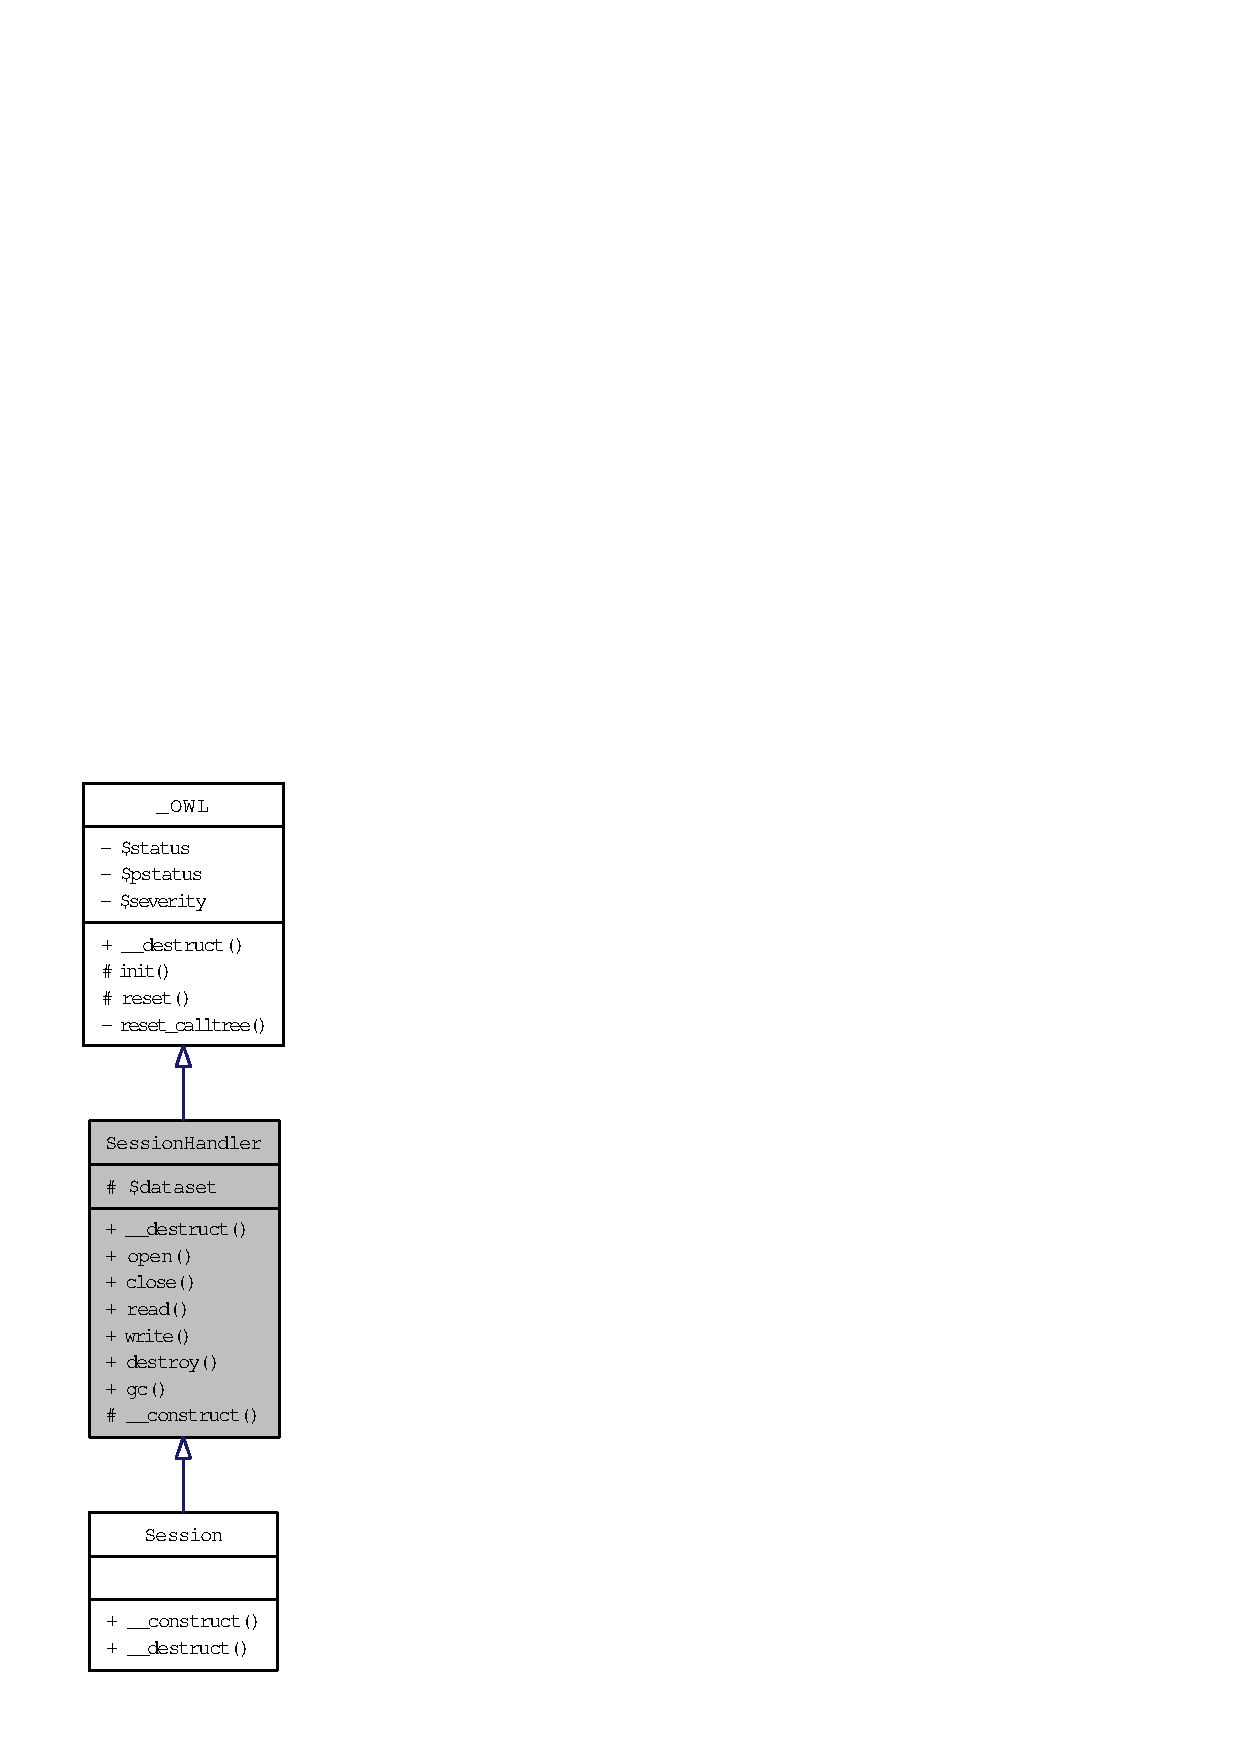
\includegraphics[width=70pt]{classSessionHandler__inherit__graph}
\end{center}
\end{figure}
Collaboration diagram for SessionHandler:\nopagebreak
\begin{figure}[H]
\begin{center}
\leavevmode
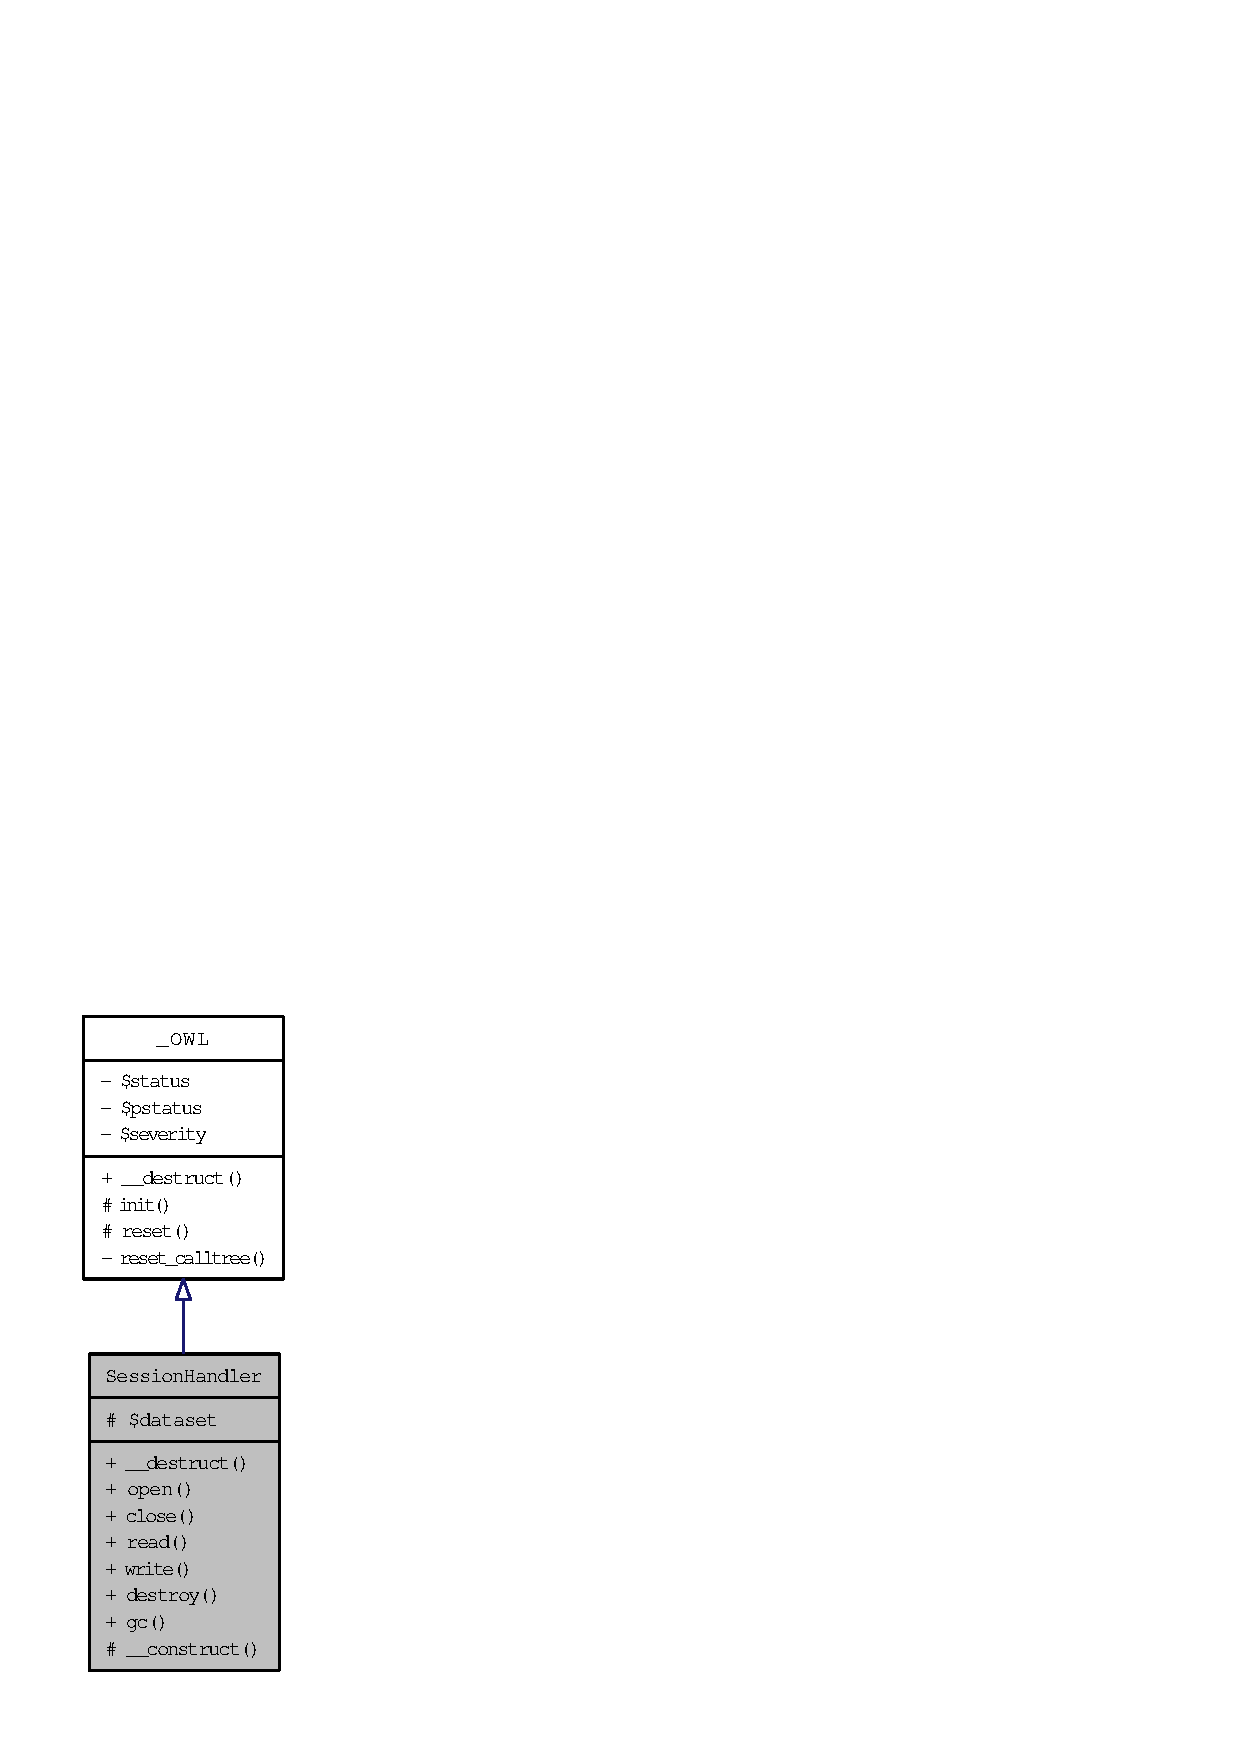
\includegraphics[width=70pt]{classSessionHandler__coll__graph}
\end{center}
\end{figure}
\subsection*{Protected Member Functions}
\begin{CompactItemize}
\item 
\hyperlink{class__OWL_e0ef3ded56e8a6b34b6461e5a721cd3e}{init} ()
\item 
\hyperlink{class__OWL_2f2a042bcf31965194c03033df0edc9b}{reset} ()
\end{CompactItemize}
\subsection*{Protected Attributes}
\begin{CompactItemize}
\item 
\hyperlink{class__OWL_f37a011667dda12fc417a68a6f3077d1}{\$config}
\end{CompactItemize}
\subsection*{Private Attributes}
\begin{CompactItemize}
\item 
\hyperlink{classSessionHandler_74c46fcfbadd4c4e6bacc73ddf350056}{\$dataset}
\end{CompactItemize}


\subsection{Detailed Description}
the PHP session object 

This class saves and (re)stores the user sessions \begin{Desc}
\item[Author:]Oscar van Eijk, Oveas Functionality Provider \end{Desc}
\begin{Desc}
\item[Version:]Jul 29, 2008 -- O van Eijk -- initial version \end{Desc}


\subsection{Member Function Documentation}
\hypertarget{class__OWL_e0ef3ded56e8a6b34b6461e5a721cd3e}{
\index{SessionHandler@{SessionHandler}!init@{init}}
\index{init@{init}!SessionHandler@{SessionHandler}}
\subsubsection{\setlength{\rightskip}{0pt plus 5cm}\_\-OWL::init ()\hspace{0.3cm}{\tt  \mbox{[}final, protected, inherited\mbox{]}}}}
\label{class__OWL_e0ef3ded56e8a6b34b6461e5a721cd3e}


This function should be called by all constuctors. It initializes the general characteristics. Status is 'warning' by default, it's up to the contructor to set a proper status; if it's still 'warning', this $\ast$might$\ast$ indicate something went wrong. \hypertarget{class__OWL_2f2a042bcf31965194c03033df0edc9b}{
\index{SessionHandler@{SessionHandler}!reset@{reset}}
\index{reset@{reset}!SessionHandler@{SessionHandler}}
\subsubsection{\setlength{\rightskip}{0pt plus 5cm}\_\-OWL::reset ()\hspace{0.3cm}{\tt  \mbox{[}protected, inherited\mbox{]}}}}
\label{class__OWL_2f2a042bcf31965194c03033df0edc9b}


General reset function for all objects. Should be called after each non-fatal error 

Reimplemented in \hyperlink{classDbHandler_9982df4830f05803935bb31bac7fae3d}{DbHandler}.

\subsection{Member Data Documentation}
\hypertarget{classSessionHandler_74c46fcfbadd4c4e6bacc73ddf350056}{
\index{SessionHandler@{SessionHandler}!\$dataset@{\$dataset}}
\index{\$dataset@{\$dataset}!SessionHandler@{SessionHandler}}
\subsubsection{\setlength{\rightskip}{0pt plus 5cm}SessionHandler::\$dataset\hspace{0.3cm}{\tt  \mbox{[}private\mbox{]}}}}
\label{classSessionHandler_74c46fcfbadd4c4e6bacc73ddf350056}


Link to a datahandler object. This dataset is used as an interface to all database IO. \hypertarget{class__OWL_f37a011667dda12fc417a68a6f3077d1}{
\index{SessionHandler@{SessionHandler}!\$config@{\$config}}
\index{\$config@{\$config}!SessionHandler@{SessionHandler}}
\subsubsection{\setlength{\rightskip}{0pt plus 5cm}\_\-OWL::\$config\hspace{0.3cm}{\tt  \mbox{[}protected, inherited\mbox{]}}}}
\label{class__OWL_f37a011667dda12fc417a68a6f3077d1}


The global Config array is referenced from every object 

The documentation for this class was generated from the following file:\begin{CompactItemize}
\item 
/home/oscar/work/eclipse/owl-php/src/inc/\hyperlink{class_8sessionhandler_8php}{class.sessionhandler.php}\end{CompactItemize}

\chapter{OWL-PHP File Documentation}
\hypertarget{config_8php}{
\section{/home/oscar/work/eclipse/owl-php/src/config.php File Reference}
\label{config_8php}\index{/home/oscar/work/eclipse/owl-php/src/config.php@{/home/oscar/work/eclipse/owl-php/src/config.php}}
}
\subsection*{Variables}
\begin{CompactItemize}
\item 
\hyperlink{config_8php_6cc1ef3a8c20d69988531d27f931855b}{\$GLOBALS} \mbox{[}'register'\mbox{]}
\item 
\hyperlink{config_8php_36e909583250c43d72bdc7c09e2d4a20}{\$GLOBALS} \mbox{[}'config'\mbox{]}\mbox{[}'configfiles'\mbox{]}\mbox{[}'owl'\mbox{]} = \hyperlink{index_8php_35612f9a6bd7277982731a74593272c4}{OWL\_\-ROOT} . '/owl\_\-config.cfg'
\item 
\hyperlink{config_8php_335a0ed5b0fc63ef47f9ba1d91e41dc6}{\$GLOBALS} \mbox{[}'config'\mbox{]}\mbox{[}'image\_\-types'\mbox{]} = '/gif/jpg/jpeg/png/swf/psd/bmp/'
\item 
\hyperlink{config_8php_93b1c5faba6a6e120b07b4206a619144}{\$GLOBALS} \mbox{[}'config'\mbox{]}\mbox{[}'archive\_\-types'\mbox{]} = '/gzip/gz/Z/zip/arj/zoo/tar/bzip2/'
\item 
\hyperlink{config_8php_bf54039b81f6214bcc39d4f399ad068f}{\$GLOBALS} \mbox{[}'config'\mbox{]}\mbox{[}'webdocument\_\-types'\mbox{]} = '/html/php/'
\item 
\hyperlink{config_8php_c4d548310cf87788e37150caed7d4092}{\$GLOBALS} \mbox{[}'config'\mbox{]}\mbox{[}'script\_\-types'\mbox{]} = '/php/'
\item 
\hyperlink{config_8php_0192eb81e0d90debab674415130b0884}{\$GLOBALS} \mbox{[}'config'\mbox{]}\mbox{[}'binary\_\-files'\mbox{]} = '/zip/gz/tar/arj/gif/jpg/jpeg/png/swf/psd/bmp/pdf/exe/'
\item 
\hyperlink{config_8php_feeb257c3edcf45093f5ffaccc3b8ee0}{\$GLOBALS} \mbox{[}'config'\mbox{]}\mbox{[}'ascii\_\-files'\mbox{]} = '/txt/html/php/js/asp/phtml/xhtml/'
\end{CompactItemize}


\subsection{Detailed Description}
Configuration basics file for OWL; it stores some fixed configuration in a global data structure \begin{Desc}
\item[Version:]\$Id\$ \end{Desc}


\subsection{Variable Documentation}
\hypertarget{config_8php_feeb257c3edcf45093f5ffaccc3b8ee0}{
\index{config.php@{config.php}!\$GLOBALS@{\$GLOBALS}}
\index{\$GLOBALS@{\$GLOBALS}!config.php@{config.php}}
\subsubsection{\setlength{\rightskip}{0pt plus 5cm}\$GLOBALS\mbox{[}'config'\mbox{]}\mbox{[}'ascii\_\-files'\mbox{]} = '/txt/html/php/js/asp/phtml/xhtml/'}}
\label{config_8php_feeb257c3edcf45093f5ffaccc3b8ee0}


\hypertarget{config_8php_0192eb81e0d90debab674415130b0884}{
\index{config.php@{config.php}!\$GLOBALS@{\$GLOBALS}}
\index{\$GLOBALS@{\$GLOBALS}!config.php@{config.php}}
\subsubsection{\setlength{\rightskip}{0pt plus 5cm}\$GLOBALS\mbox{[}'config'\mbox{]}\mbox{[}'binary\_\-files'\mbox{]} = '/zip/gz/tar/arj/gif/jpg/jpeg/png/swf/psd/bmp/pdf/exe/'}}
\label{config_8php_0192eb81e0d90debab674415130b0884}


\hypertarget{config_8php_c4d548310cf87788e37150caed7d4092}{
\index{config.php@{config.php}!\$GLOBALS@{\$GLOBALS}}
\index{\$GLOBALS@{\$GLOBALS}!config.php@{config.php}}
\subsubsection{\setlength{\rightskip}{0pt plus 5cm}\$GLOBALS\mbox{[}'config'\mbox{]}\mbox{[}'script\_\-types'\mbox{]} = '/php/'}}
\label{config_8php_c4d548310cf87788e37150caed7d4092}


\hypertarget{config_8php_bf54039b81f6214bcc39d4f399ad068f}{
\index{config.php@{config.php}!\$GLOBALS@{\$GLOBALS}}
\index{\$GLOBALS@{\$GLOBALS}!config.php@{config.php}}
\subsubsection{\setlength{\rightskip}{0pt plus 5cm}\$GLOBALS\mbox{[}'config'\mbox{]}\mbox{[}'webdocument\_\-types'\mbox{]} = '/html/php/'}}
\label{config_8php_bf54039b81f6214bcc39d4f399ad068f}


\hypertarget{config_8php_93b1c5faba6a6e120b07b4206a619144}{
\index{config.php@{config.php}!\$GLOBALS@{\$GLOBALS}}
\index{\$GLOBALS@{\$GLOBALS}!config.php@{config.php}}
\subsubsection{\setlength{\rightskip}{0pt plus 5cm}\$GLOBALS\mbox{[}'config'\mbox{]}\mbox{[}'archive\_\-types'\mbox{]} = '/gzip/gz/Z/zip/arj/zoo/tar/bzip2/'}}
\label{config_8php_93b1c5faba6a6e120b07b4206a619144}


\hypertarget{config_8php_335a0ed5b0fc63ef47f9ba1d91e41dc6}{
\index{config.php@{config.php}!\$GLOBALS@{\$GLOBALS}}
\index{\$GLOBALS@{\$GLOBALS}!config.php@{config.php}}
\subsubsection{\setlength{\rightskip}{0pt plus 5cm}\$GLOBALS\mbox{[}'config'\mbox{]}\mbox{[}'image\_\-types'\mbox{]} = '/gif/jpg/jpeg/png/swf/psd/bmp/'}}
\label{config_8php_335a0ed5b0fc63ef47f9ba1d91e41dc6}


\hypertarget{config_8php_36e909583250c43d72bdc7c09e2d4a20}{
\index{config.php@{config.php}!\$GLOBALS@{\$GLOBALS}}
\index{\$GLOBALS@{\$GLOBALS}!config.php@{config.php}}
\subsubsection{\setlength{\rightskip}{0pt plus 5cm}\$GLOBALS\mbox{[}'config'\mbox{]}\mbox{[}'configfiles'\mbox{]}\mbox{[}'owl'\mbox{]} = {\bf OWL\_\-ROOT} . '/owl\_\-config.cfg'}}
\label{config_8php_36e909583250c43d72bdc7c09e2d4a20}


\hypertarget{config_8php_6cc1ef3a8c20d69988531d27f931855b}{
\index{config.php@{config.php}!\$GLOBALS@{\$GLOBALS}}
\index{\$GLOBALS@{\$GLOBALS}!config.php@{config.php}}
\subsubsection{\setlength{\rightskip}{0pt plus 5cm}\$GLOBALS\mbox{[}'register'\mbox{]}}}
\label{config_8php_6cc1ef3a8c20d69988531d27f931855b}


\textbf{Initial value:}

\begin{Code}\begin{verbatim} array (
                                          'applications'        => array()
                                        , 'classes'                     => array()
                                )
\end{verbatim}
\end{Code}

\hypertarget{class_8__OWL_8php}{
\section{/home/oscar/work/eclipse/owl-php/src/inc/class.\_\-OWL.php File Reference}
\label{class_8__OWL_8php}\index{/home/oscar/work/eclipse/owl-php/src/inc/class.\_\-OWL.php@{/home/oscar/work/eclipse/owl-php/src/inc/class.\_\-OWL.php}}
}
\subsection*{Classes}
\begin{CompactItemize}
\item 
class \hyperlink{class__OWL}{\_\-OWL}
\end{CompactItemize}


\subsection{Detailed Description}
This file defines the Oveas Web Library main class \begin{Desc}
\item[Version:]\end{Desc}
\begin{Desc}
\item[Id]\hyperlink{class_8__OWL_8php}{class.\_\-OWL.php},v 1.1 2008-08-07 10:21:21 oscar Exp \end{Desc}

\hypertarget{class_8datahandler_8php}{
\section{/home/oscar/work/eclipse/owl-php/src/kernel/so/class.datahandler.php File Reference}
\label{class_8datahandler_8php}\index{/home/oscar/work/eclipse/owl-php/src/kernel/so/class.datahandler.php@{/home/oscar/work/eclipse/owl-php/src/kernel/so/class.datahandler.php}}
}
\subsection*{Classes}
\begin{CompactItemize}
\item 
class \hyperlink{classDataHandler}{DataHandler}
\begin{CompactList}\small\item\em The \hyperlink{classOWL}{OWL} Data object. \item\end{CompactList}\end{CompactItemize}
\subsection*{Enumerations}
\begin{Indent}{\bf Query preparation tools}\par
{\em These flags define what type of queries can be prepared }\begin{CompactItemize}
\item 
enum \hyperlink{class_8datahandler_8php_21c8184f96d445f8f608321e0e8fffc9}{DATA\_\-UNPREPARED} 
\begin{CompactList}\small\item\em Default value; no query prepared yet. \item\end{CompactList}\item 
enum \hyperlink{class_8datahandler_8php_c28f74b49007773d24ca2207baac6d32}{DATA\_\-READ} 
\begin{CompactList}\small\item\em Read data from the database. \item\end{CompactList}\item 
enum \hyperlink{class_8datahandler_8php_5d8b54a2eb4767a05a2e577c2db9193a}{DATA\_\-WRITE} 
\begin{CompactList}\small\item\em Write new data to the database. \item\end{CompactList}\item 
enum \hyperlink{class_8datahandler_8php_9a817a8e9190bfc1eb884f9b4c3cb7c8}{DATA\_\-UPDATE} 
\begin{CompactList}\small\item\em Update data in the database. \item\end{CompactList}\item 
enum \hyperlink{class_8datahandler_8php_b4fa180fa2d24c38e425ff9ca4c913fa}{DATA\_\-DELETE} 
\begin{CompactList}\small\item\em Remove data from the database. \item\end{CompactList}\end{CompactItemize}
\end{Indent}
\begin{Indent}{\bf Reset flags}\par
{\em These flags how an object should be performed. All values includes all lower values as well! }\begin{CompactItemize}
\item 
enum \hyperlink{class_8datahandler_8php_9266811d651cb3ff8c5fdf00111e677b}{DATA\_\-RESET\_\-STATUS} 
\begin{CompactList}\small\item\em Reset object status only. \item\end{CompactList}\item 
enum \hyperlink{class_8datahandler_8php_19a99423705b41e563424ae76d7fe184}{DATA\_\-RESET\_\-PREPARE} 
\begin{CompactList}\small\item\em Reset prepared queries as well. \item\end{CompactList}\item 
enum \hyperlink{class_8datahandler_8php_3ce9f928f9ba75096925bd4157246bbb}{DATA\_\-RESET\_\-META} 
\begin{CompactList}\small\item\em Remove all locks and joins. \item\end{CompactList}\item 
enum \hyperlink{class_8datahandler_8php_2a28429433990da242faa223d5a49f0a}{DATA\_\-RESET\_\-FULL} 
\begin{CompactList}\small\item\em Clean all data. \item\end{CompactList}\end{CompactItemize}
\end{Indent}


\subsection{Detailed Description}
This file defines the \hyperlink{classDataHandler}{DataHandler} class \begin{Desc}
\item[Version:]\end{Desc}
\begin{Desc}
\item[Id]\hyperlink{class_8datahandler_8php}{class.datahandler.php},v 1.2 2008-08-28 18:12:52 oscar Exp \end{Desc}


\subsection{Enumeration Type Documentation}
\hypertarget{class_8datahandler_8php_b4fa180fa2d24c38e425ff9ca4c913fa}{
\index{class.datahandler.php@{class.datahandler.php}!DATA\_\-DELETE@{DATA\_\-DELETE}}
\index{DATA\_\-DELETE@{DATA\_\-DELETE}!class.datahandler.php@{class.datahandler.php}}
\subsubsection{\setlength{\rightskip}{0pt plus 5cm}enum {\bf DATA\_\-DELETE}}}
\label{class_8datahandler_8php_b4fa180fa2d24c38e425ff9ca4c913fa}


Remove data from the database. 

\hypertarget{class_8datahandler_8php_c28f74b49007773d24ca2207baac6d32}{
\index{class.datahandler.php@{class.datahandler.php}!DATA\_\-READ@{DATA\_\-READ}}
\index{DATA\_\-READ@{DATA\_\-READ}!class.datahandler.php@{class.datahandler.php}}
\subsubsection{\setlength{\rightskip}{0pt plus 5cm}enum {\bf DATA\_\-READ}}}
\label{class_8datahandler_8php_c28f74b49007773d24ca2207baac6d32}


Read data from the database. 

\hypertarget{class_8datahandler_8php_2a28429433990da242faa223d5a49f0a}{
\index{class.datahandler.php@{class.datahandler.php}!DATA\_\-RESET\_\-FULL@{DATA\_\-RESET\_\-FULL}}
\index{DATA\_\-RESET\_\-FULL@{DATA\_\-RESET\_\-FULL}!class.datahandler.php@{class.datahandler.php}}
\subsubsection{\setlength{\rightskip}{0pt plus 5cm}enum {\bf DATA\_\-RESET\_\-FULL}}}
\label{class_8datahandler_8php_2a28429433990da242faa223d5a49f0a}


Clean all data. 

\hypertarget{class_8datahandler_8php_3ce9f928f9ba75096925bd4157246bbb}{
\index{class.datahandler.php@{class.datahandler.php}!DATA\_\-RESET\_\-META@{DATA\_\-RESET\_\-META}}
\index{DATA\_\-RESET\_\-META@{DATA\_\-RESET\_\-META}!class.datahandler.php@{class.datahandler.php}}
\subsubsection{\setlength{\rightskip}{0pt plus 5cm}enum {\bf DATA\_\-RESET\_\-META}}}
\label{class_8datahandler_8php_3ce9f928f9ba75096925bd4157246bbb}


Remove all locks and joins. 

\hypertarget{class_8datahandler_8php_19a99423705b41e563424ae76d7fe184}{
\index{class.datahandler.php@{class.datahandler.php}!DATA\_\-RESET\_\-PREPARE@{DATA\_\-RESET\_\-PREPARE}}
\index{DATA\_\-RESET\_\-PREPARE@{DATA\_\-RESET\_\-PREPARE}!class.datahandler.php@{class.datahandler.php}}
\subsubsection{\setlength{\rightskip}{0pt plus 5cm}enum {\bf DATA\_\-RESET\_\-PREPARE}}}
\label{class_8datahandler_8php_19a99423705b41e563424ae76d7fe184}


Reset prepared queries as well. 

\hypertarget{class_8datahandler_8php_9266811d651cb3ff8c5fdf00111e677b}{
\index{class.datahandler.php@{class.datahandler.php}!DATA\_\-RESET\_\-STATUS@{DATA\_\-RESET\_\-STATUS}}
\index{DATA\_\-RESET\_\-STATUS@{DATA\_\-RESET\_\-STATUS}!class.datahandler.php@{class.datahandler.php}}
\subsubsection{\setlength{\rightskip}{0pt plus 5cm}enum {\bf DATA\_\-RESET\_\-STATUS}}}
\label{class_8datahandler_8php_9266811d651cb3ff8c5fdf00111e677b}


Reset object status only. 

\hypertarget{class_8datahandler_8php_21c8184f96d445f8f608321e0e8fffc9}{
\index{class.datahandler.php@{class.datahandler.php}!DATA\_\-UNPREPARED@{DATA\_\-UNPREPARED}}
\index{DATA\_\-UNPREPARED@{DATA\_\-UNPREPARED}!class.datahandler.php@{class.datahandler.php}}
\subsubsection{\setlength{\rightskip}{0pt plus 5cm}enum {\bf DATA\_\-UNPREPARED}}}
\label{class_8datahandler_8php_21c8184f96d445f8f608321e0e8fffc9}


Default value; no query prepared yet. 

\hypertarget{class_8datahandler_8php_9a817a8e9190bfc1eb884f9b4c3cb7c8}{
\index{class.datahandler.php@{class.datahandler.php}!DATA\_\-UPDATE@{DATA\_\-UPDATE}}
\index{DATA\_\-UPDATE@{DATA\_\-UPDATE}!class.datahandler.php@{class.datahandler.php}}
\subsubsection{\setlength{\rightskip}{0pt plus 5cm}enum {\bf DATA\_\-UPDATE}}}
\label{class_8datahandler_8php_9a817a8e9190bfc1eb884f9b4c3cb7c8}


Update data in the database. 

\hypertarget{class_8datahandler_8php_5d8b54a2eb4767a05a2e577c2db9193a}{
\index{class.datahandler.php@{class.datahandler.php}!DATA\_\-WRITE@{DATA\_\-WRITE}}
\index{DATA\_\-WRITE@{DATA\_\-WRITE}!class.datahandler.php@{class.datahandler.php}}
\subsubsection{\setlength{\rightskip}{0pt plus 5cm}enum {\bf DATA\_\-WRITE}}}
\label{class_8datahandler_8php_5d8b54a2eb4767a05a2e577c2db9193a}


Write new data to the database. 


\section{/home/oscar/projects/owl-\/php/src/kernel/so/class.dbhandler.php File Reference}
\label{class_8dbhandler_8php}\index{/home/oscar/projects/owl-\/php/src/kernel/so/class.dbhandler.php@{/home/oscar/projects/owl-\/php/src/kernel/so/class.dbhandler.php}}
\subsection*{Classes}
\begin{DoxyCompactItemize}
\item 
class {\bf DbHandler}
\begin{DoxyCompactList}\small\item\em Database handler. \end{DoxyCompactList}\end{DoxyCompactItemize}
\subsection*{Enumerations}
\begin{DoxyCompactItemize}
\item 
enum {\bf DBHANDLE\_\-DATA} 
\begin{DoxyCompactList}\small\item\em Return the read values (default) \end{DoxyCompactList}\item 
enum {\bf DBHANDLE\_\-SINGLEFIELD} 
\begin{DoxyCompactList}\small\item\em Return the read value as a single field (i.s.o. a 2D array) \end{DoxyCompactList}\item 
enum {\bf DBHANDLE\_\-SINGLEROW} 
\begin{DoxyCompactList}\small\item\em Return the read value as a single row (a 1D array) \end{DoxyCompactList}\item 
enum {\bf DBHANDLE\_\-ROWCOUNT} 
\begin{DoxyCompactList}\small\item\em Return the number of rows. \end{DoxyCompactList}\item 
enum {\bf DBHANDLE\_\-FIELDCOUNT} 
\begin{DoxyCompactList}\small\item\em Return the number of fields per row. \end{DoxyCompactList}\item 
enum {\bf DBHANDLE\_\-TOTALFIELDCOUNT} 
\begin{DoxyCompactList}\small\item\em Return the total number of fields. \end{DoxyCompactList}\item 
enum {\bf DBHANDLE\_\-READ} 
\begin{DoxyCompactList}\small\item\em Read data from the database. \end{DoxyCompactList}\item 
enum {\bf DBHANDLE\_\-INSERT} 
\begin{DoxyCompactList}\small\item\em Write new data to the database. \end{DoxyCompactList}\item 
enum {\bf DBHANDLE\_\-UPDATE} 
\begin{DoxyCompactList}\small\item\em Update data in the database. \end{DoxyCompactList}\item 
enum {\bf DBHANDLE\_\-DELETE} 
\begin{DoxyCompactList}\small\item\em Remove data from the database. \end{DoxyCompactList}\item 
enum {\bf DBHANDLE\_\-FAILED} 
\begin{DoxyCompactList}\small\item\em Last prepare action failed. \end{DoxyCompactList}\item 
enum {\bf DBHANDLE\_\-COMPLETED} 
\begin{DoxyCompactList}\small\item\em Last prepared query was executed. Chect object staus for the result. \end{DoxyCompactList}\item 
enum {\bf DBMATCH\_\-EQ} 
\begin{DoxyCompactList}\small\item\em Left and right values should match (default) (when the value contains percent signs, 'LIKE' will be used;. \end{DoxyCompactList}\item 
enum {\bf DBMATCH\_\-LT} 
\begin{DoxyCompactList}\small\item\em Left value should be less than right value. \end{DoxyCompactList}\item 
enum {\bf DBMATCH\_\-GT} 
\begin{DoxyCompactList}\small\item\em Left value should be greater than right value. \end{DoxyCompactList}\item 
enum {\bf DBMATCH\_\-LE} 
\begin{DoxyCompactList}\small\item\em Left value should be less than or equal to right value. \end{DoxyCompactList}\item 
enum {\bf DBMATCH\_\-GE} 
\begin{DoxyCompactList}\small\item\em Left value should be greater than or equal to right value. \end{DoxyCompactList}\item 
enum {\bf DBMATCH\_\-NONE} 
\begin{DoxyCompactList}\small\item\em Don't match on this field, use it in the SELECT list instead. \end{DoxyCompactList}\end{DoxyCompactItemize}


\subsection{Detailed Description}
This file defines the Database Handler class \begin{DoxyAuthor}{Author}
Oscar van Eijk, Oveas Functionality Provider 
\end{DoxyAuthor}
\begin{DoxyVersion}{Version}

\end{DoxyVersion}
\begin{DoxyParagraph}{Id:}
\doxyref{class.dbhandler.php}{p.}{class_8dbhandler_8php},v 1.28 2011-\/05-\/26 12:26:30 oscar Exp 
\end{DoxyParagraph}

\section{/home/oscar/projects/owl-\/php/src/kernel/so/class.filehandler.php File Reference}
\label{class_8filehandler_8php}\index{/home/oscar/projects/owl-\/php/src/kernel/so/class.filehandler.php@{/home/oscar/projects/owl-\/php/src/kernel/so/class.filehandler.php}}
\subsection*{Classes}
\begin{DoxyCompactItemize}
\item 
class {\bf FileHandler}
\begin{DoxyCompactList}\small\item\em File handler. \end{DoxyCompactList}\item 
class {\bf OldOFMStuff}
\end{DoxyCompactItemize}
\subsection*{Enumerations}
\begin{Indent}\paragraph*{Dataline trim flags}
{\em These flags define how datalines should be trimmed when read from a file }\begin{DoxyCompactItemize}
\item 
enum {\bf FILE\_\-NOTRIM} 
\begin{DoxyCompactList}\small\item\em Don't trim. \end{DoxyCompactList}\item 
enum {\bf FILE\_\-TRIM\_\-L} 
\begin{DoxyCompactList}\small\item\em Trim left part of a line read. \end{DoxyCompactList}\item 
enum {\bf FILE\_\-TRIM\_\-R} 
\begin{DoxyCompactList}\small\item\em Trim right part of a line read. \end{DoxyCompactList}\item 
enum {\bf FILE\_\-TRIM\_\-C} 
\begin{DoxyCompactList}\small\item\em Replace all multiple spaces in a line read with a single space. \end{DoxyCompactList}\end{DoxyCompactItemize}
\end{Indent}


\subsection{Detailed Description}
This file defines the \doxyref{FileHandler}{p.}{classFileHandler} class \begin{DoxyVersion}{Version}

\end{DoxyVersion}
\begin{DoxyParagraph}{Id:}
\doxyref{class.filehandler.php}{p.}{class_8filehandler_8php},v 1.5 2010-\/12-\/03 12:07:42 oscar Exp 
\end{DoxyParagraph}


\subsection{Enumeration Type Documentation}
\index{class.filehandler.php@{class.filehandler.php}!FILE\_\-NOTRIM@{FILE\_\-NOTRIM}}
\index{FILE\_\-NOTRIM@{FILE\_\-NOTRIM}!class.filehandler.php@{class.filehandler.php}}
\subsubsection[{FILE\_\-NOTRIM}]{\setlength{\rightskip}{0pt plus 5cm}enum {\bf FILE\_\-NOTRIM}}\label{class_8filehandler_8php_a3720f2e15eb9e16e29d8ecbb96763662}


Don't trim. 

\index{class.filehandler.php@{class.filehandler.php}!FILE\_\-TRIM\_\-C@{FILE\_\-TRIM\_\-C}}
\index{FILE\_\-TRIM\_\-C@{FILE\_\-TRIM\_\-C}!class.filehandler.php@{class.filehandler.php}}
\subsubsection[{FILE\_\-TRIM\_\-C}]{\setlength{\rightskip}{0pt plus 5cm}enum {\bf FILE\_\-TRIM\_\-C}}\label{class_8filehandler_8php_a2787c3a1ecef8697c863800d0b2848a4}


Replace all multiple spaces in a line read with a single space. 

\index{class.filehandler.php@{class.filehandler.php}!FILE\_\-TRIM\_\-L@{FILE\_\-TRIM\_\-L}}
\index{FILE\_\-TRIM\_\-L@{FILE\_\-TRIM\_\-L}!class.filehandler.php@{class.filehandler.php}}
\subsubsection[{FILE\_\-TRIM\_\-L}]{\setlength{\rightskip}{0pt plus 5cm}enum {\bf FILE\_\-TRIM\_\-L}}\label{class_8filehandler_8php_a080de95fd7cf2e8d8ac78ac7ad9471ee}


Trim left part of a line read. 

\index{class.filehandler.php@{class.filehandler.php}!FILE\_\-TRIM\_\-R@{FILE\_\-TRIM\_\-R}}
\index{FILE\_\-TRIM\_\-R@{FILE\_\-TRIM\_\-R}!class.filehandler.php@{class.filehandler.php}}
\subsubsection[{FILE\_\-TRIM\_\-R}]{\setlength{\rightskip}{0pt plus 5cm}enum {\bf FILE\_\-TRIM\_\-R}}\label{class_8filehandler_8php_a7ee25ec88036b90f5a0ae8be7bc41769}


Trim right part of a line read. 


\section{/home/oscar/projects/owl-\/php/src/kernel/so/class.sessionhandler.php File Reference}
\label{class_8sessionhandler_8php}\index{/home/oscar/projects/owl-\/php/src/kernel/so/class.sessionhandler.php@{/home/oscar/projects/owl-\/php/src/kernel/so/class.sessionhandler.php}}
\subsection*{Classes}
\begin{DoxyCompactItemize}
\item 
class {\bf SessionHandler}
\begin{DoxyCompactList}\small\item\em the PHP session object \end{DoxyCompactList}\end{DoxyCompactItemize}
\subsection*{Enumerations}
\begin{DoxyCompactItemize}
\item 
enum {\bf SESSIONVAR\_\-SET} 
\begin{DoxyCompactList}\small\item\em Set variable to the given value (default) \end{DoxyCompactList}\item 
enum {\bf SESSIONVAR\_\-UNSET} 
\begin{DoxyCompactList}\small\item\em Unset the variable. \end{DoxyCompactList}\item 
enum {\bf SESSIONVAR\_\-INCR} 
\begin{DoxyCompactList}\small\item\em Increase the variable or set as the given value if not yet existing. \end{DoxyCompactList}\item 
enum {\bf SESSIONVAR\_\-DECR} 
\begin{DoxyCompactList}\small\item\em Decrease the variable or set as the given value if not yet existing. \end{DoxyCompactList}\item 
enum {\bf SESSIONVAR\_\-ARRAY} 
\begin{DoxyCompactList}\small\item\em Add the variable to an array. If a value already exists, it will be the first element. \end{DoxyCompactList}\end{DoxyCompactItemize}


\subsection{Detailed Description}
This file defines the \doxyref{SessionHandler}{p.}{classSessionHandler} class \begin{DoxyAuthor}{Author}
Oscar van Eijk, Oveas Functionality Provider 
\end{DoxyAuthor}
\begin{DoxyVersion}{Version}

\end{DoxyVersion}
\begin{DoxyParagraph}{Id:}
\doxyref{class.sessionhandler.php}{p.}{class_8sessionhandler_8php},v 1.15 2011-\/05-\/02 12:56:13 oscar Exp 
\end{DoxyParagraph}

\hypertarget{index_8php}{
\section{/home/oscar/work/eclipse/owl-php/src/index.php File Reference}
\label{index_8php}\index{/home/oscar/work/eclipse/owl-php/src/index.php@{/home/oscar/work/eclipse/owl-php/src/index.php}}
}
\subsection*{Enumerations}
\begin{CompactItemize}
\item 
enum \hyperlink{index_8php_35612f9a6bd7277982731a74593272c4}{OWL\_\-ROOT} 
\item 
enum \hyperlink{index_8php_4d33a8f2fcc9c83cbeea921c4cb23a7f}{OWL\_\-INCLUDE} 
\item 
enum \hyperlink{index_8php_74eed08508c8b70677c4167acf49e427}{OWL\_\-LIBRARY} 
\end{CompactItemize}
\subsection*{Variables}
\begin{CompactItemize}
\item 
\hyperlink{index_8php_14159e18d9b64fd1e16054f784eda311}{\$GLOBALS} \mbox{[}'db'\mbox{]}
\item 
\hyperlink{index_8php_df2bd79dcae941587d8b69d6ece9104a}{\$GLOBALS} \mbox{[}'sessiondata'\mbox{]} = \& new \hyperlink{classDataHandler}{DataHandler} (\&\$GLOBALS\mbox{[}'db'\mbox{]})
\item 
\hyperlink{index_8php_95ec104c636100b9022c09964e2b0725}{\$GLOBALS} \mbox{[}'session'\mbox{]} = \& new \hyperlink{classSessionHandler}{SessionHandler}(\&\$GLOBALS\mbox{[}'sessiondata'\mbox{]})
\end{CompactItemize}


\subsection{Detailed Description}
This is the entry point for OWL-PHP teststub \begin{Desc}
\item[Version:]\$Id\$ \end{Desc}


\subsection{Enumeration Type Documentation}
\hypertarget{index_8php_4d33a8f2fcc9c83cbeea921c4cb23a7f}{
\index{index.php@{index.php}!OWL\_\-INCLUDE@{OWL\_\-INCLUDE}}
\index{OWL\_\-INCLUDE@{OWL\_\-INCLUDE}!index.php@{index.php}}
\subsubsection{\setlength{\rightskip}{0pt plus 5cm}enum {\bf OWL\_\-INCLUDE}}}
\label{index_8php_4d33a8f2fcc9c83cbeea921c4cb23a7f}


\hypertarget{index_8php_74eed08508c8b70677c4167acf49e427}{
\index{index.php@{index.php}!OWL\_\-LIBRARY@{OWL\_\-LIBRARY}}
\index{OWL\_\-LIBRARY@{OWL\_\-LIBRARY}!index.php@{index.php}}
\subsubsection{\setlength{\rightskip}{0pt plus 5cm}enum {\bf OWL\_\-LIBRARY}}}
\label{index_8php_74eed08508c8b70677c4167acf49e427}


\hypertarget{index_8php_35612f9a6bd7277982731a74593272c4}{
\index{index.php@{index.php}!OWL\_\-ROOT@{OWL\_\-ROOT}}
\index{OWL\_\-ROOT@{OWL\_\-ROOT}!index.php@{index.php}}
\subsubsection{\setlength{\rightskip}{0pt plus 5cm}enum {\bf OWL\_\-ROOT}}}
\label{index_8php_35612f9a6bd7277982731a74593272c4}




\subsection{Variable Documentation}
\hypertarget{index_8php_95ec104c636100b9022c09964e2b0725}{
\index{index.php@{index.php}!\$GLOBALS@{\$GLOBALS}}
\index{\$GLOBALS@{\$GLOBALS}!index.php@{index.php}}
\subsubsection{\setlength{\rightskip}{0pt plus 5cm}\$GLOBALS\mbox{[}'session'\mbox{]} = \& new {\bf SessionHandler}(\&\$GLOBALS\mbox{[}'sessiondata'\mbox{]})}}
\label{index_8php_95ec104c636100b9022c09964e2b0725}


\hypertarget{index_8php_df2bd79dcae941587d8b69d6ece9104a}{
\index{index.php@{index.php}!\$GLOBALS@{\$GLOBALS}}
\index{\$GLOBALS@{\$GLOBALS}!index.php@{index.php}}
\subsubsection{\setlength{\rightskip}{0pt plus 5cm}\$GLOBALS\mbox{[}'sessiondata'\mbox{]} = \& new {\bf DataHandler} (\&\$GLOBALS\mbox{[}'db'\mbox{]})}}
\label{index_8php_df2bd79dcae941587d8b69d6ece9104a}


\hypertarget{index_8php_14159e18d9b64fd1e16054f784eda311}{
\index{index.php@{index.php}!\$GLOBALS@{\$GLOBALS}}
\index{\$GLOBALS@{\$GLOBALS}!index.php@{index.php}}
\subsubsection{\setlength{\rightskip}{0pt plus 5cm}\$GLOBALS\mbox{[}'db'\mbox{]}}}
\label{index_8php_14159e18d9b64fd1e16054f784eda311}


\textbf{Initial value:}

\begin{Code}\begin{verbatim}& new DBHandler(
                          $GLOBALS['config']['dbserver']
                        , $GLOBALS['config']['dbname']
                        , $GLOBALS['config']['dbuser']
                        , $GLOBALS['config']['dbpasswd'])
\end{verbatim}
\end{Code}

\hypertarget{owl_8messages_8en-uk_8php}{
\section{/home/oscar/work/eclipse/owl-php/src/lib/owl.messages.en-uk.php File Reference}
\label{owl_8messages_8en-uk_8php}\index{/home/oscar/work/eclipse/owl-php/src/lib/owl.messages.en-uk.php@{/home/oscar/work/eclipse/owl-php/src/lib/owl.messages.en-uk.php}}
}
\subsection*{Variables}
\begin{CompactItemize}
\item 
\hyperlink{owl_8messages_8en-uk_8php_65f2996116eed36e9ab25f254a470259}{\$GLOBALS} \mbox{[}'messages'\mbox{]}
\end{CompactItemize}


\subsection{Detailed Description}
This file defines the message text for all status codes in UK English \begin{Desc}
\item[Version:]\end{Desc}
\begin{Desc}
\item[Id]owl.messages.en-uk.php,v 1.4 2008-09-02 05:16:54 oscar Exp \end{Desc}


\subsection{Variable Documentation}
\hypertarget{owl_8messages_8en-uk_8php_65f2996116eed36e9ab25f254a470259}{
\index{owl.messages.en-uk.php@{owl.messages.en-uk.php}!\$GLOBALS@{\$GLOBALS}}
\index{\$GLOBALS@{\$GLOBALS}!owl.messages.en-uk.php@{owl.messages.en-uk.php}}
\subsubsection{\setlength{\rightskip}{0pt plus 5cm}\$GLOBALS\mbox{[}'messages'\mbox{]}}}
\label{owl_8messages_8en-uk_8php_65f2996116eed36e9ab25f254a470259}



\section{/home/oscar/projects/owl-\/php/src/lib/owl.severitycodes.php File Reference}
\label{owl_8severitycodes_8php}\index{/home/oscar/projects/owl-\/php/src/lib/owl.severitycodes.php@{/home/oscar/projects/owl-\/php/src/lib/owl.severitycodes.php}}
\subsection*{Enumerations}
\begin{DoxyCompactItemize}
\item 
enum {\bf OWL\_\-DEBUG} 
\item 
enum {\bf OWL\_\-INFO} 
\item 
enum {\bf OWL\_\-OK} 
\item 
enum {\bf OWL\_\-SUCCESS} 
\item 
enum {\bf OWL\_\-WARNING} 
\item 
enum {\bf OWL\_\-BUG} 
\item 
enum {\bf OWL\_\-ERROR} 
\item 
enum {\bf OWL\_\-FATAL} 
\item 
enum {\bf OWL\_\-CRITICAL} 
\end{DoxyCompactItemize}


\subsection{Detailed Description}
This file defines the Severity codes that all objects can have. It must be the very first file that is inluded, since these codes are used from step 1. \begin{DoxyAuthor}{Author}
Oscar van Eijk, Oveas Functionality Provider 
\end{DoxyAuthor}
\begin{DoxyVersion}{Version}

\end{DoxyVersion}
\begin{DoxyParagraph}{Id:}
\doxyref{owl.severitycodes.php}{p.}{owl_8severitycodes_8php},v 1.3 2011-\/05-\/02 12:56:14 oscar Exp 
\end{DoxyParagraph}

\hypertarget{owl_8statuscodes_8php}{
\section{/home/oscar/work/eclipse/owl-php/src/lib/owl.statuscodes.php File Reference}
\label{owl_8statuscodes_8php}\index{/home/oscar/work/eclipse/owl-php/src/lib/owl.statuscodes.php@{/home/oscar/work/eclipse/owl-php/src/lib/owl.statuscodes.php}}
}
\subsection*{Enumerations}
\begin{Indent}{\bf }\par
\begin{CompactItemize}
\item 
enum \hyperlink{owl_8statuscodes_8php_8bbae521b65a3416f22e2879c911de3f}{OWL\_\-STATUS\_\-OK} 
\item 
enum \hyperlink{owl_8statuscodes_8php_783f6a33a00386bc20447487bc76c94e}{OWL\_\-STATUS\_\-WARNING} 
\item 
enum \hyperlink{owl_8statuscodes_8php_b00c7cf8190cde5630604617b408ce71}{OWL\_\-STATUS\_\-ERROR} 
\item 
enum \hyperlink{owl_8statuscodes_8php_d3a24b224b20a07e626894d7da745455}{OWL\_\-STATUS\_\-BUG} 
\item 
enum \hyperlink{owl_8statuscodes_8php_3e17ae43daac1a9847afaf18ae02b5f6}{OWL\_\-STATUS\_\-FNF} 
\item 
enum \hyperlink{owl_8statuscodes_8php_b67c4e6fe36a5f763d59e49ee1395a6e}{OWL\_\-STATUS\_\-ROPENERR} 
\item 
enum \hyperlink{owl_8statuscodes_8php_9d2015fb92c189204f143b637398f40c}{OWL\_\-STATUS\_\-WOPENERR} 
\item 
enum \hyperlink{owl_8statuscodes_8php_3b2d7ec8e84f7022afe7dc2c9f96e964}{OWL\_\-STATUS\_\-NOKEY} 
\item 
enum \hyperlink{owl_8statuscodes_8php_c0fd62708c370d17b251339d38cc92ca}{OWL\_\-STATUS\_\-IVKEY} 
\end{CompactItemize}
\end{Indent}
\begin{Indent}{\bf }\par
\begin{CompactItemize}
\item 
enum \hyperlink{owl_8statuscodes_8php_9d228a8481d3e68d6c8034fd41e1284f}{SESSION\_\-INVUSERNAME} 
\item 
enum \hyperlink{owl_8statuscodes_8php_61e828f14b93df840752f73190104a50}{SESSION\_\-NODATASET} 
\item 
enum \hyperlink{owl_8statuscodes_8php_44b42092523fa97db313970c190ea28b}{SESSION\_\-INVPASSWORD} 
\item 
enum \hyperlink{owl_8statuscodes_8php_9f864ccc821ad3799322c4a6793796dc}{SESSION\_\-TIMEOUT} 
\item 
enum \hyperlink{owl_8statuscodes_8php_a1062a5298847727e0d3be4eab23d210}{SESSION\_\-NOACCESS} 
\item 
enum \hyperlink{owl_8statuscodes_8php_776112495f2ed2c5e256dcdfad21fe7e}{SESSION\_\-DISABLED} 
\item 
enum \hyperlink{owl_8statuscodes_8php_9897ac79456358fa862ca33fdea13bb9}{SESSION\_\-IVSESSION} 
\end{CompactItemize}
\end{Indent}
\begin{Indent}{\bf }\par
\begin{CompactItemize}
\item 
enum \hyperlink{owl_8statuscodes_8php_9a343c4560417e293caa709e22646196}{DBHANDLE\_\-CONNECTERR} 
\item 
enum \hyperlink{owl_8statuscodes_8php_b64cc6f10455b678241bc8b714100e16}{DBHANDLE\_\-OPENERR} 
\item 
enum \hyperlink{owl_8statuscodes_8php_ab8d7571a5e75d71060fbcb865433490}{DBHANDLE\_\-DBCLOSED} 
\item 
enum \hyperlink{owl_8statuscodes_8php_04ae2b6da16ff57c8c425aa57561b030}{DBHANDLE\_\-QUERYERR} 
\item 
enum \hyperlink{owl_8statuscodes_8php_e18225c004a543b76af09a71c10a8f4f}{DBHANDLE\_\-CREATERR} 
\item 
enum \hyperlink{owl_8statuscodes_8php_d8e472506309827bb507ccf4f1545e0e}{DBHANDLE\_\-NODATA} 
\item 
enum \hyperlink{owl_8statuscodes_8php_6d2955056daf49887e50eea132eb595e}{DBHANDLE\_\-IVTABLE} 
\end{CompactItemize}
\end{Indent}
\begin{Indent}{\bf }\par
\begin{CompactItemize}
\item 
enum \hyperlink{owl_8statuscodes_8php_1b3920489f064605aec419c2f18a43c6}{DATA\_\-NOTFOUND} 
\item 
enum \hyperlink{owl_8statuscodes_8php_d2b2ac63774859fb01412dcf1d416a30}{DATA\_\-NOSELECT} 
\item 
enum \hyperlink{owl_8statuscodes_8php_de36d7efad634ceb46de1b6670e6af08}{DATA\_\-IVARRAY} 
\item 
enum \hyperlink{owl_8statuscodes_8php_4567c5a928f00431e3c61ed317494ad1}{DATA\_\-AMBFIELD} 
\item 
enum \hyperlink{owl_8statuscodes_8php_f5b9acbc941403d2077e28968a8ad3fc}{DATA\_\-NODBLINK} 
\item 
enum \hyperlink{owl_8statuscodes_8php_ef494323f427edd5668413ba3ae3e4c0}{DATA\_\-IVPREPARE} 
\item 
enum \hyperlink{owl_8statuscodes_8php_86d2cc4775b7b6282502b36048984a24}{DATA\_\-IVRESET} 
\end{CompactItemize}
\end{Indent}
\begin{Indent}{\bf }\par
\begin{CompactItemize}
\item 
enum \hyperlink{owl_8statuscodes_8php_a5abc6e073dcb61147f56d7854983787}{FILE\_\-NOSUCHFILE} 
\item 
enum \hyperlink{owl_8statuscodes_8php_c0e1f657ef7713fe45084b10af74670b}{FILE\_\-ENDOFFILE} 
\item 
enum \hyperlink{owl_8statuscodes_8php_3abc0dabe8ead6f76dd62c3e2b506af7}{FILE\_\-OPENOPENED} 
\item 
enum \hyperlink{owl_8statuscodes_8php_ce4541108274f542d69d8fa4523e13f6}{FILE\_\-CLOSECLOSED} 
\item 
enum \hyperlink{owl_8statuscodes_8php_d540d25f34464adfbce1258d9a37fe3f}{FILE\_\-OPENERR} 
\end{CompactItemize}
\end{Indent}


\subsection{Detailed Description}
This file defines the Status codes that all objects can have. \begin{Desc}
\item[Version:]\$Id\$ \end{Desc}


\subsection{Enumeration Type Documentation}
\hypertarget{owl_8statuscodes_8php_4567c5a928f00431e3c61ed317494ad1}{
\index{owl.statuscodes.php@{owl.statuscodes.php}!DATA\_\-AMBFIELD@{DATA\_\-AMBFIELD}}
\index{DATA\_\-AMBFIELD@{DATA\_\-AMBFIELD}!owl.statuscodes.php@{owl.statuscodes.php}}
\subsubsection{\setlength{\rightskip}{0pt plus 5cm}enum {\bf DATA\_\-AMBFIELD}}}
\label{owl_8statuscodes_8php_4567c5a928f00431e3c61ed317494ad1}


\hypertarget{owl_8statuscodes_8php_de36d7efad634ceb46de1b6670e6af08}{
\index{owl.statuscodes.php@{owl.statuscodes.php}!DATA\_\-IVARRAY@{DATA\_\-IVARRAY}}
\index{DATA\_\-IVARRAY@{DATA\_\-IVARRAY}!owl.statuscodes.php@{owl.statuscodes.php}}
\subsubsection{\setlength{\rightskip}{0pt plus 5cm}enum {\bf DATA\_\-IVARRAY}}}
\label{owl_8statuscodes_8php_de36d7efad634ceb46de1b6670e6af08}


\hypertarget{owl_8statuscodes_8php_ef494323f427edd5668413ba3ae3e4c0}{
\index{owl.statuscodes.php@{owl.statuscodes.php}!DATA\_\-IVPREPARE@{DATA\_\-IVPREPARE}}
\index{DATA\_\-IVPREPARE@{DATA\_\-IVPREPARE}!owl.statuscodes.php@{owl.statuscodes.php}}
\subsubsection{\setlength{\rightskip}{0pt plus 5cm}enum {\bf DATA\_\-IVPREPARE}}}
\label{owl_8statuscodes_8php_ef494323f427edd5668413ba3ae3e4c0}


\hypertarget{owl_8statuscodes_8php_86d2cc4775b7b6282502b36048984a24}{
\index{owl.statuscodes.php@{owl.statuscodes.php}!DATA\_\-IVRESET@{DATA\_\-IVRESET}}
\index{DATA\_\-IVRESET@{DATA\_\-IVRESET}!owl.statuscodes.php@{owl.statuscodes.php}}
\subsubsection{\setlength{\rightskip}{0pt plus 5cm}enum {\bf DATA\_\-IVRESET}}}
\label{owl_8statuscodes_8php_86d2cc4775b7b6282502b36048984a24}


\hypertarget{owl_8statuscodes_8php_f5b9acbc941403d2077e28968a8ad3fc}{
\index{owl.statuscodes.php@{owl.statuscodes.php}!DATA\_\-NODBLINK@{DATA\_\-NODBLINK}}
\index{DATA\_\-NODBLINK@{DATA\_\-NODBLINK}!owl.statuscodes.php@{owl.statuscodes.php}}
\subsubsection{\setlength{\rightskip}{0pt plus 5cm}enum {\bf DATA\_\-NODBLINK}}}
\label{owl_8statuscodes_8php_f5b9acbc941403d2077e28968a8ad3fc}


\hypertarget{owl_8statuscodes_8php_d2b2ac63774859fb01412dcf1d416a30}{
\index{owl.statuscodes.php@{owl.statuscodes.php}!DATA\_\-NOSELECT@{DATA\_\-NOSELECT}}
\index{DATA\_\-NOSELECT@{DATA\_\-NOSELECT}!owl.statuscodes.php@{owl.statuscodes.php}}
\subsubsection{\setlength{\rightskip}{0pt plus 5cm}enum {\bf DATA\_\-NOSELECT}}}
\label{owl_8statuscodes_8php_d2b2ac63774859fb01412dcf1d416a30}


\hypertarget{owl_8statuscodes_8php_1b3920489f064605aec419c2f18a43c6}{
\index{owl.statuscodes.php@{owl.statuscodes.php}!DATA\_\-NOTFOUND@{DATA\_\-NOTFOUND}}
\index{DATA\_\-NOTFOUND@{DATA\_\-NOTFOUND}!owl.statuscodes.php@{owl.statuscodes.php}}
\subsubsection{\setlength{\rightskip}{0pt plus 5cm}enum {\bf DATA\_\-NOTFOUND}}}
\label{owl_8statuscodes_8php_1b3920489f064605aec419c2f18a43c6}


Data error- codes \hypertarget{owl_8statuscodes_8php_9a343c4560417e293caa709e22646196}{
\index{owl.statuscodes.php@{owl.statuscodes.php}!DBHANDLE\_\-CONNECTERR@{DBHANDLE\_\-CONNECTERR}}
\index{DBHANDLE\_\-CONNECTERR@{DBHANDLE\_\-CONNECTERR}!owl.statuscodes.php@{owl.statuscodes.php}}
\subsubsection{\setlength{\rightskip}{0pt plus 5cm}enum {\bf DBHANDLE\_\-CONNECTERR}}}
\label{owl_8statuscodes_8php_9a343c4560417e293caa709e22646196}


MySQL error-codes \hypertarget{owl_8statuscodes_8php_e18225c004a543b76af09a71c10a8f4f}{
\index{owl.statuscodes.php@{owl.statuscodes.php}!DBHANDLE\_\-CREATERR@{DBHANDLE\_\-CREATERR}}
\index{DBHANDLE\_\-CREATERR@{DBHANDLE\_\-CREATERR}!owl.statuscodes.php@{owl.statuscodes.php}}
\subsubsection{\setlength{\rightskip}{0pt plus 5cm}enum {\bf DBHANDLE\_\-CREATERR}}}
\label{owl_8statuscodes_8php_e18225c004a543b76af09a71c10a8f4f}


\hypertarget{owl_8statuscodes_8php_ab8d7571a5e75d71060fbcb865433490}{
\index{owl.statuscodes.php@{owl.statuscodes.php}!DBHANDLE\_\-DBCLOSED@{DBHANDLE\_\-DBCLOSED}}
\index{DBHANDLE\_\-DBCLOSED@{DBHANDLE\_\-DBCLOSED}!owl.statuscodes.php@{owl.statuscodes.php}}
\subsubsection{\setlength{\rightskip}{0pt plus 5cm}enum {\bf DBHANDLE\_\-DBCLOSED}}}
\label{owl_8statuscodes_8php_ab8d7571a5e75d71060fbcb865433490}


\hypertarget{owl_8statuscodes_8php_6d2955056daf49887e50eea132eb595e}{
\index{owl.statuscodes.php@{owl.statuscodes.php}!DBHANDLE\_\-IVTABLE@{DBHANDLE\_\-IVTABLE}}
\index{DBHANDLE\_\-IVTABLE@{DBHANDLE\_\-IVTABLE}!owl.statuscodes.php@{owl.statuscodes.php}}
\subsubsection{\setlength{\rightskip}{0pt plus 5cm}enum {\bf DBHANDLE\_\-IVTABLE}}}
\label{owl_8statuscodes_8php_6d2955056daf49887e50eea132eb595e}


\hypertarget{owl_8statuscodes_8php_d8e472506309827bb507ccf4f1545e0e}{
\index{owl.statuscodes.php@{owl.statuscodes.php}!DBHANDLE\_\-NODATA@{DBHANDLE\_\-NODATA}}
\index{DBHANDLE\_\-NODATA@{DBHANDLE\_\-NODATA}!owl.statuscodes.php@{owl.statuscodes.php}}
\subsubsection{\setlength{\rightskip}{0pt plus 5cm}enum {\bf DBHANDLE\_\-NODATA}}}
\label{owl_8statuscodes_8php_d8e472506309827bb507ccf4f1545e0e}


\hypertarget{owl_8statuscodes_8php_b64cc6f10455b678241bc8b714100e16}{
\index{owl.statuscodes.php@{owl.statuscodes.php}!DBHANDLE\_\-OPENERR@{DBHANDLE\_\-OPENERR}}
\index{DBHANDLE\_\-OPENERR@{DBHANDLE\_\-OPENERR}!owl.statuscodes.php@{owl.statuscodes.php}}
\subsubsection{\setlength{\rightskip}{0pt plus 5cm}enum {\bf DBHANDLE\_\-OPENERR}}}
\label{owl_8statuscodes_8php_b64cc6f10455b678241bc8b714100e16}


\hypertarget{owl_8statuscodes_8php_04ae2b6da16ff57c8c425aa57561b030}{
\index{owl.statuscodes.php@{owl.statuscodes.php}!DBHANDLE\_\-QUERYERR@{DBHANDLE\_\-QUERYERR}}
\index{DBHANDLE\_\-QUERYERR@{DBHANDLE\_\-QUERYERR}!owl.statuscodes.php@{owl.statuscodes.php}}
\subsubsection{\setlength{\rightskip}{0pt plus 5cm}enum {\bf DBHANDLE\_\-QUERYERR}}}
\label{owl_8statuscodes_8php_04ae2b6da16ff57c8c425aa57561b030}


\hypertarget{owl_8statuscodes_8php_ce4541108274f542d69d8fa4523e13f6}{
\index{owl.statuscodes.php@{owl.statuscodes.php}!FILE\_\-CLOSECLOSED@{FILE\_\-CLOSECLOSED}}
\index{FILE\_\-CLOSECLOSED@{FILE\_\-CLOSECLOSED}!owl.statuscodes.php@{owl.statuscodes.php}}
\subsubsection{\setlength{\rightskip}{0pt plus 5cm}enum {\bf FILE\_\-CLOSECLOSED}}}
\label{owl_8statuscodes_8php_ce4541108274f542d69d8fa4523e13f6}


\hypertarget{owl_8statuscodes_8php_c0e1f657ef7713fe45084b10af74670b}{
\index{owl.statuscodes.php@{owl.statuscodes.php}!FILE\_\-ENDOFFILE@{FILE\_\-ENDOFFILE}}
\index{FILE\_\-ENDOFFILE@{FILE\_\-ENDOFFILE}!owl.statuscodes.php@{owl.statuscodes.php}}
\subsubsection{\setlength{\rightskip}{0pt plus 5cm}enum {\bf FILE\_\-ENDOFFILE}}}
\label{owl_8statuscodes_8php_c0e1f657ef7713fe45084b10af74670b}


\hypertarget{owl_8statuscodes_8php_a5abc6e073dcb61147f56d7854983787}{
\index{owl.statuscodes.php@{owl.statuscodes.php}!FILE\_\-NOSUCHFILE@{FILE\_\-NOSUCHFILE}}
\index{FILE\_\-NOSUCHFILE@{FILE\_\-NOSUCHFILE}!owl.statuscodes.php@{owl.statuscodes.php}}
\subsubsection{\setlength{\rightskip}{0pt plus 5cm}enum {\bf FILE\_\-NOSUCHFILE}}}
\label{owl_8statuscodes_8php_a5abc6e073dcb61147f56d7854983787}


Fileobject and -system error-codes \hypertarget{owl_8statuscodes_8php_d540d25f34464adfbce1258d9a37fe3f}{
\index{owl.statuscodes.php@{owl.statuscodes.php}!FILE\_\-OPENERR@{FILE\_\-OPENERR}}
\index{FILE\_\-OPENERR@{FILE\_\-OPENERR}!owl.statuscodes.php@{owl.statuscodes.php}}
\subsubsection{\setlength{\rightskip}{0pt plus 5cm}enum {\bf FILE\_\-OPENERR}}}
\label{owl_8statuscodes_8php_d540d25f34464adfbce1258d9a37fe3f}


\hypertarget{owl_8statuscodes_8php_3abc0dabe8ead6f76dd62c3e2b506af7}{
\index{owl.statuscodes.php@{owl.statuscodes.php}!FILE\_\-OPENOPENED@{FILE\_\-OPENOPENED}}
\index{FILE\_\-OPENOPENED@{FILE\_\-OPENOPENED}!owl.statuscodes.php@{owl.statuscodes.php}}
\subsubsection{\setlength{\rightskip}{0pt plus 5cm}enum {\bf FILE\_\-OPENOPENED}}}
\label{owl_8statuscodes_8php_3abc0dabe8ead6f76dd62c3e2b506af7}


\hypertarget{owl_8statuscodes_8php_d3a24b224b20a07e626894d7da745455}{
\index{owl.statuscodes.php@{owl.statuscodes.php}!OWL\_\-STATUS\_\-BUG@{OWL\_\-STATUS\_\-BUG}}
\index{OWL\_\-STATUS\_\-BUG@{OWL\_\-STATUS\_\-BUG}!owl.statuscodes.php@{owl.statuscodes.php}}
\subsubsection{\setlength{\rightskip}{0pt plus 5cm}enum {\bf OWL\_\-STATUS\_\-BUG}}}
\label{owl_8statuscodes_8php_d3a24b224b20a07e626894d7da745455}


\hypertarget{owl_8statuscodes_8php_b00c7cf8190cde5630604617b408ce71}{
\index{owl.statuscodes.php@{owl.statuscodes.php}!OWL\_\-STATUS\_\-ERROR@{OWL\_\-STATUS\_\-ERROR}}
\index{OWL\_\-STATUS\_\-ERROR@{OWL\_\-STATUS\_\-ERROR}!owl.statuscodes.php@{owl.statuscodes.php}}
\subsubsection{\setlength{\rightskip}{0pt plus 5cm}enum {\bf OWL\_\-STATUS\_\-ERROR}}}
\label{owl_8statuscodes_8php_b00c7cf8190cde5630604617b408ce71}


\hypertarget{owl_8statuscodes_8php_3e17ae43daac1a9847afaf18ae02b5f6}{
\index{owl.statuscodes.php@{owl.statuscodes.php}!OWL\_\-STATUS\_\-FNF@{OWL\_\-STATUS\_\-FNF}}
\index{OWL\_\-STATUS\_\-FNF@{OWL\_\-STATUS\_\-FNF}!owl.statuscodes.php@{owl.statuscodes.php}}
\subsubsection{\setlength{\rightskip}{0pt plus 5cm}enum {\bf OWL\_\-STATUS\_\-FNF}}}
\label{owl_8statuscodes_8php_3e17ae43daac1a9847afaf18ae02b5f6}


\hypertarget{owl_8statuscodes_8php_c0fd62708c370d17b251339d38cc92ca}{
\index{owl.statuscodes.php@{owl.statuscodes.php}!OWL\_\-STATUS\_\-IVKEY@{OWL\_\-STATUS\_\-IVKEY}}
\index{OWL\_\-STATUS\_\-IVKEY@{OWL\_\-STATUS\_\-IVKEY}!owl.statuscodes.php@{owl.statuscodes.php}}
\subsubsection{\setlength{\rightskip}{0pt plus 5cm}enum {\bf OWL\_\-STATUS\_\-IVKEY}}}
\label{owl_8statuscodes_8php_c0fd62708c370d17b251339d38cc92ca}


\hypertarget{owl_8statuscodes_8php_3b2d7ec8e84f7022afe7dc2c9f96e964}{
\index{owl.statuscodes.php@{owl.statuscodes.php}!OWL\_\-STATUS\_\-NOKEY@{OWL\_\-STATUS\_\-NOKEY}}
\index{OWL\_\-STATUS\_\-NOKEY@{OWL\_\-STATUS\_\-NOKEY}!owl.statuscodes.php@{owl.statuscodes.php}}
\subsubsection{\setlength{\rightskip}{0pt plus 5cm}enum {\bf OWL\_\-STATUS\_\-NOKEY}}}
\label{owl_8statuscodes_8php_3b2d7ec8e84f7022afe7dc2c9f96e964}


\hypertarget{owl_8statuscodes_8php_8bbae521b65a3416f22e2879c911de3f}{
\index{owl.statuscodes.php@{owl.statuscodes.php}!OWL\_\-STATUS\_\-OK@{OWL\_\-STATUS\_\-OK}}
\index{OWL\_\-STATUS\_\-OK@{OWL\_\-STATUS\_\-OK}!owl.statuscodes.php@{owl.statuscodes.php}}
\subsubsection{\setlength{\rightskip}{0pt plus 5cm}enum {\bf OWL\_\-STATUS\_\-OK}}}
\label{owl_8statuscodes_8php_8bbae521b65a3416f22e2879c911de3f}


General used status codes \hypertarget{owl_8statuscodes_8php_b67c4e6fe36a5f763d59e49ee1395a6e}{
\index{owl.statuscodes.php@{owl.statuscodes.php}!OWL\_\-STATUS\_\-ROPENERR@{OWL\_\-STATUS\_\-ROPENERR}}
\index{OWL\_\-STATUS\_\-ROPENERR@{OWL\_\-STATUS\_\-ROPENERR}!owl.statuscodes.php@{owl.statuscodes.php}}
\subsubsection{\setlength{\rightskip}{0pt plus 5cm}enum {\bf OWL\_\-STATUS\_\-ROPENERR}}}
\label{owl_8statuscodes_8php_b67c4e6fe36a5f763d59e49ee1395a6e}


\hypertarget{owl_8statuscodes_8php_783f6a33a00386bc20447487bc76c94e}{
\index{owl.statuscodes.php@{owl.statuscodes.php}!OWL\_\-STATUS\_\-WARNING@{OWL\_\-STATUS\_\-WARNING}}
\index{OWL\_\-STATUS\_\-WARNING@{OWL\_\-STATUS\_\-WARNING}!owl.statuscodes.php@{owl.statuscodes.php}}
\subsubsection{\setlength{\rightskip}{0pt plus 5cm}enum {\bf OWL\_\-STATUS\_\-WARNING}}}
\label{owl_8statuscodes_8php_783f6a33a00386bc20447487bc76c94e}


\hypertarget{owl_8statuscodes_8php_9d2015fb92c189204f143b637398f40c}{
\index{owl.statuscodes.php@{owl.statuscodes.php}!OWL\_\-STATUS\_\-WOPENERR@{OWL\_\-STATUS\_\-WOPENERR}}
\index{OWL\_\-STATUS\_\-WOPENERR@{OWL\_\-STATUS\_\-WOPENERR}!owl.statuscodes.php@{owl.statuscodes.php}}
\subsubsection{\setlength{\rightskip}{0pt plus 5cm}enum {\bf OWL\_\-STATUS\_\-WOPENERR}}}
\label{owl_8statuscodes_8php_9d2015fb92c189204f143b637398f40c}


\hypertarget{owl_8statuscodes_8php_776112495f2ed2c5e256dcdfad21fe7e}{
\index{owl.statuscodes.php@{owl.statuscodes.php}!SESSION\_\-DISABLED@{SESSION\_\-DISABLED}}
\index{SESSION\_\-DISABLED@{SESSION\_\-DISABLED}!owl.statuscodes.php@{owl.statuscodes.php}}
\subsubsection{\setlength{\rightskip}{0pt plus 5cm}enum {\bf SESSION\_\-DISABLED}}}
\label{owl_8statuscodes_8php_776112495f2ed2c5e256dcdfad21fe7e}


\hypertarget{owl_8statuscodes_8php_44b42092523fa97db313970c190ea28b}{
\index{owl.statuscodes.php@{owl.statuscodes.php}!SESSION\_\-INVPASSWORD@{SESSION\_\-INVPASSWORD}}
\index{SESSION\_\-INVPASSWORD@{SESSION\_\-INVPASSWORD}!owl.statuscodes.php@{owl.statuscodes.php}}
\subsubsection{\setlength{\rightskip}{0pt plus 5cm}enum {\bf SESSION\_\-INVPASSWORD}}}
\label{owl_8statuscodes_8php_44b42092523fa97db313970c190ea28b}


\hypertarget{owl_8statuscodes_8php_9d228a8481d3e68d6c8034fd41e1284f}{
\index{owl.statuscodes.php@{owl.statuscodes.php}!SESSION\_\-INVUSERNAME@{SESSION\_\-INVUSERNAME}}
\index{SESSION\_\-INVUSERNAME@{SESSION\_\-INVUSERNAME}!owl.statuscodes.php@{owl.statuscodes.php}}
\subsubsection{\setlength{\rightskip}{0pt plus 5cm}enum {\bf SESSION\_\-INVUSERNAME}}}
\label{owl_8statuscodes_8php_9d228a8481d3e68d6c8034fd41e1284f}


Session error- codes \hypertarget{owl_8statuscodes_8php_9897ac79456358fa862ca33fdea13bb9}{
\index{owl.statuscodes.php@{owl.statuscodes.php}!SESSION\_\-IVSESSION@{SESSION\_\-IVSESSION}}
\index{SESSION\_\-IVSESSION@{SESSION\_\-IVSESSION}!owl.statuscodes.php@{owl.statuscodes.php}}
\subsubsection{\setlength{\rightskip}{0pt plus 5cm}enum {\bf SESSION\_\-IVSESSION}}}
\label{owl_8statuscodes_8php_9897ac79456358fa862ca33fdea13bb9}


\hypertarget{owl_8statuscodes_8php_a1062a5298847727e0d3be4eab23d210}{
\index{owl.statuscodes.php@{owl.statuscodes.php}!SESSION\_\-NOACCESS@{SESSION\_\-NOACCESS}}
\index{SESSION\_\-NOACCESS@{SESSION\_\-NOACCESS}!owl.statuscodes.php@{owl.statuscodes.php}}
\subsubsection{\setlength{\rightskip}{0pt plus 5cm}enum {\bf SESSION\_\-NOACCESS}}}
\label{owl_8statuscodes_8php_a1062a5298847727e0d3be4eab23d210}


\hypertarget{owl_8statuscodes_8php_61e828f14b93df840752f73190104a50}{
\index{owl.statuscodes.php@{owl.statuscodes.php}!SESSION\_\-NODATASET@{SESSION\_\-NODATASET}}
\index{SESSION\_\-NODATASET@{SESSION\_\-NODATASET}!owl.statuscodes.php@{owl.statuscodes.php}}
\subsubsection{\setlength{\rightskip}{0pt plus 5cm}enum {\bf SESSION\_\-NODATASET}}}
\label{owl_8statuscodes_8php_61e828f14b93df840752f73190104a50}


\hypertarget{owl_8statuscodes_8php_9f864ccc821ad3799322c4a6793796dc}{
\index{owl.statuscodes.php@{owl.statuscodes.php}!SESSION\_\-TIMEOUT@{SESSION\_\-TIMEOUT}}
\index{SESSION\_\-TIMEOUT@{SESSION\_\-TIMEOUT}!owl.statuscodes.php@{owl.statuscodes.php}}
\subsubsection{\setlength{\rightskip}{0pt plus 5cm}enum {\bf SESSION\_\-TIMEOUT}}}
\label{owl_8statuscodes_8php_9f864ccc821ad3799322c4a6793796dc}



\printindex
\end{document}
